%% 
%% Copyright 2007-2025 Elsevier Ltd
%% 
%% This file is part of the 'Elsarticle Bundle'.
%% ---------------------------------------------
%% 
%% It may be distributed under the conditions of the LaTeX Project Public
%% License, either version 1.3 of this license or (at your option) any
%% later version.  The latest version of this license is in
%%    http://www.latex-project.org/lppl.txt
%% and version 1.3 or later is part of all distributions of LaTeX
%% version 1999/12/01 or later.
%% 
%% The list of all files belonging to the 'Elsarticle Bundle' is
%% given in the file `manifest.txt'.
%% 
%% Template article for Elsevier's document class `elsarticle'
%% with numbered style bibliographic references
%% SP 2008/03/01
%% $Id: elsarticle-template-num.tex 272 2025-01-09 17:36:26Z rishi $
%%
%\documentclass[preprint,12pt]{elsarticle}

%% Use the option review to obtain double line spacing
%\documentclass[authoryear, final, 12pt]{elsarticle} %review, 
%\documentclass[final,1p,times,twocolumn]{elsarticle}
\documentclass[review, authoryear, 1p]{elsarticle} %review, 

%% Use the options 1p,twocolumn; 3p; 3p,twocolumn; 5p; or 5p,twocolumn
%% for a journal layout:
%\documentclass[final,1p,times]{elsarticle}
%% \documentclass[final,1p,times,twocolumn]{elsarticle}
%% \documentclass[final,3p,times]{elsarticle}
%% \documentclass[final,3p,times,twocolumn]{elsarticle}
%% \documentclass[final,5p,times]{elsarticle}
%% \documentclass[final,5p,times,twocolumn]{elsarticle}

%% For including figures, graphicx.sty has been loaded in
%% elsarticle.cls. If you prefer to use the old commands
%% please give \usepackage{epsfig}

%% The amssymb package provides various useful mathematical symbols
\usepackage{amssymb}
%% The amsmath package provides various useful equation environments.
\usepackage{amsmath}
%% The amsthm package provides extended theorem environments
%% \usepackage{amsthm}
\usepackage{hyperref}
%\usepackage{lineno}
% User-added packages
\usepackage{listings}
\usepackage{array}
\usepackage{xcolor}
\usepackage{soul}
\usepackage{booktabs}
%\usepackage{manyfoot}%
%\usepackage{footnote}
%\makesavenoteenv{tabular}  % if using footnotes inside tabular
\usepackage{tabularx}
\usepackage{geometry}
\usepackage{threeparttable}
\usepackage[nolist]{acronym}
\usepackage[figuresright]{rotating} % include this in your preamble
\usepackage{adjustbox}
\usepackage{tablefootnote}

\usepackage[utf8]{inputenc}   % ensures proper UTF-8 handling
\usepackage[T1]{fontenc}      % modern font encoding
\usepackage{textcomp} 

\usepackage{threeparttable}
\usepackage{enumitem}

% Define a muted color palette
\definecolor{codebg}{RGB}{253, 253, 253}
\definecolor{keywordcolor}{RGB}{30,60,114}
\definecolor{stringcolor}{RGB}{50,100,50}
\definecolor{commentcolor}{RGB}{150,150,150}
\definecolor{identifiercolor}{RGB}{40,40,40}
\definecolor{codegreen}{rgb}{0,0.6,0}
\definecolor{codegray}{rgb}{0.5,0.5,0.5}
\definecolor{codepurple}{rgb}{0.58,0,0.82}
\definecolor{backcolour}{rgb}{0.95,0.95,0.92}
\definecolor{darkred}{rgb}{0.6,0.0,0.0}
\definecolor{darkgreen}{rgb}{0,0.50,0}
\definecolor{lightblue}{rgb}{0.0,0.42,0.91}
\definecolor{orange}{rgb}{0.99,0.48,0.13}
\definecolor{grass}{rgb}{0.18,0.80,0.18}
\definecolor{pink}{rgb}{0.97,0.15,0.45}

% Custom command definitions
%\newcommand*{\figref}[2][]{%
%  \hyperref[{#2}]{%
%    \ref*{#2}%
%    \ifx\\#1\\%
%    \else
%      #1%
%    \fi
%  }%
%}

% General Setting of listings
\lstset{
  aboveskip=1em,
  breaklines=true,
  abovecaptionskip=6pt,
  captionpos=b,
  escapeinside={\%*}{*)},
  frame=single,
  numbers=left,
  numbersep=10pt,
  tabsize=2,
  keepspaces=true,                                    
  showspaces=false,                
  showstringspaces=false,
  showtabs=false,
  numberstyle=\tiny,
  breakatwhitespace=false,         
  breaklines=true,
  basicstyle=\ttfamily, %\footnotesize
}
% 1. General Python Keywords List
\lstdefinelanguage{PythonReemission}[]{Python}{
  morekeywords=[1]{,as,assert,nonlocal,with,yield,self,True,False,None,} % Python builtin
  morekeywords=[2]{,__init__,__add__,__mul__,__div__,__sub__,__call__,__getitem__,__setitem__,__eq__,__ne__,__nonzero__,__rmul__,__radd__,__repr__,__str__,__get__,__truediv__,__pow__,__name__,__future__,__all__,}, % magic methods
  morekeywords=[3]{,object,type,isinstance,copy,deepcopy,zip,enumerate,reversed,list,set,len,dict,tuple,range,xrange,append,execfile,real,imag,reduce,str,repr,}, % common functions
  morekeywords=[4]{,Exception,NameError,IndexError,SyntaxError,TypeError,ValueError,OverflowError,ZeroDivisionError,}, % errors
  morekeywords=[5]{,ode,fsolve,sqrt,exp,sin,cos,arctan,arctan2,arccos,pi, array,norm,solve,dot,arange,isscalar,max,sum,flatten,shape,reshape,find,any,all,abs,plot,linspace,legend,quad,polyval,polyfit,hstack,concatenate,vstack,column_stack,empty,zeros,ones,rand,vander,grid,pcolor,eig,eigs,eigvals,svd,qr,tan,det,logspace,roll,min,mean,cumsum,cumprod,diff,vectorize,lstsq,cla,eye,xlabel,ylabel,squeeze,},
  emph={,ReemissionEngine, MonthlyTemperature, CarbonDioxideEmission, NitrousOxideEmission, MethaneEmission, Landuse, Climate, SoilType, Biome, TreatmentFactor, LanduseIntensity, Catchment, Reservoir, BiogenicFactors}, % numpy / math
}

% 3. Extended theme
\lstdefinestyle{colorEX}{
  basicstyle=\ttfamily\footnotesize,
  backgroundcolor=\color{codebg},
  commentstyle=\color{darkgreen}\slshape,
  keywordstyle=\color{blue}\bfseries\itshape,
  keywordstyle=[2]\color{blue}\bfseries,
  keywordstyle=[3]\color{grass},
  keywordstyle=[4]\color{red},
  keywordstyle=[5]\color{orange},
  stringstyle=\color{darkred},
  emphstyle=\color{pink}\underbar,
  numberstyle=\tiny\color{codegray},
  numbersep=10pt,
}
\lstdefinestyle{custmpythonstyle}{
    backgroundcolor=\color{codebg},
    commentstyle=\color{commentcolor}\itshape,
    keywordstyle=\color{keywordcolor}\bfseries,
    stringstyle=\color{stringcolor},
    identifierstyle=\color{identifiercolor},
    breaklines=true,
    captionpos=b,
    keepspaces=true,
    numbers=left,
    frame=single,
    numbersep=10pt,
    rulecolor=\color{gray},
    showstringspaces=false
}

\lstdefinelanguage{Dockerfile}{
  morekeywords={FROM, RUN, CMD, LABEL, MAINTAINER, EXPOSE, ENV, ADD, COPY, ENTRYPOINT, VOLUME, USER, WORKDIR, ARG, ONBUILD, STOPSIGNAL, HEALTHCHECK, SHELL},
  sensitive=true,
  morecomment=[l]{\#},
  morestring=[b]"
}

\lstset{style=colorEX}

%% The lineno packages adds line numbers. Start line numbering with
%% \begin{linenumbers}, end it with \end{linenumbers}. Or switch it on
%% for the whole article with \linenumbers.
%% \usepackage{lineno}

\usepackage{caption}
\captionsetup[lstlisting]{font=small}
\captionsetup[table]{font=normalsize}
\captionsetup[figure]{font=normalsize}
\captionsetup[bibliography]{font=normalsize}

\usepackage[linesnumbered,ruled,vlined]{algorithm2e}

\usepackage{refcount}  % for \getrefnumber
\usepackage{xparse}    % for optional arguments
\NewDocumentCommand{\figref}{O{}m}{%
  \hyperref[#2]{\ref*{#2}#1}%
}

%\NewDocumentCommand{\figref}{O{}m}{%
%  \getrefnumber{#2}#1%
%}

% This will be executed when \appendix is called
\AtBeginDocument{%
  \let\oldappendix\appendix
  \renewcommand{\appendix}{%
    \oldappendix
    % Reset counters
    \setcounter{figure}{0}
    \setcounter{table}{0}
    \setcounter{equation}{0}
    \setcounter{lstlisting}{0}
    
    % Redefine the counter representation
    \renewcommand{\thefigure}{A.\arabic{figure}}
    \renewcommand{\thetable}{A.\arabic{table}}
	\renewcommand{\theequation}{A.\arabic{equation}}
    \renewcommand{\thelstlisting}{A.\arabic{lstlisting}}
  }
}

\makeatletter
\newcommand{\vrbbrk}[1]{%
  \begingroup
  \ttfamily
  \begingroup\lccode`~=`/\lowercase{\endgroup\def~}{/\discretionary{}{}{}}%
  \begingroup\lccode`~=`[\lowercase{\endgroup\def~}{[\discretionary{}{}{}}%
  \begingroup\lccode`~=`.\lowercase{\endgroup\def~}{.\discretionary{}{}{}}%
  \catcode`/=\active\catcode`[=\active\catcode`.=\active
  \scantokens{#1\noexpand}%
  \endgroup
}
\makeatother


\journal{Environmental Modelling \& Software}

\begin{document}

%\linenumbers

\begin{frontmatter}

%% Title, authors and addresses

%% use the tnoteref command within \title for footnotes;
%% use the tnotetext command for theassociated footnote;
%% use the fnref command within \author or \affiliation for footnotes;
%% use the fntext command for theassociated footnote;
%% use the corref command within \author for corresponding author footnotes;
%% use the cortext command for theassociated footnote;
%% use the ead command for the email address,
%% and the form \ead[url] for the home page:
%% \title{Title\tnoteref{label1}}
%% \tnotetext[label1]{}
%% \author{Name\corref{cor1}\fnref{label2}}
%% \ead{email address}
%% \ead[url]{home page}
%% \fntext[label2]{}
%% \cortext[cor1]{}
%% \affiliation{organization={},
%%             addressline={},
%%             city={},
%%             postcode={},
%%             state={},
%%             country={}}
%% \fntext[label3]{}

\title{\emph{Re-Emission}: A free open-source software for estimating, reporting, and visualizing greenhouse gas emissions from reservoirs}

%% use optional labels to link authors explicitly to addresses:
 \author[label1]{Tomasz Janus}
 \affiliation[label1]{organization={Tyndall Centre Manchester, University of Manchester},
             addressline={Floor 5, Engineering A, Booth Street East},
             city={Manchester},
             postcode={M13 9PL},
             %state={},
             country={United Kingdom}}
 \author[label2]{Christopher Barry}
 \affiliation[label2]{organization={UK Centre for Ecology \& Hydrology},
             addressline={Deiniol Road},
             city={Bangor},
             postcode={LL57 2UW},
             %state={},
             country={United Kingdom}}           
 \author[label3,label4]{Xingxing Zhang}
 \affiliation[label3]{organization={State Key Laboratory of Resources and Environmental Information System, Institute of Geographic Sciences and Natural Resources Research},
             addressline={Chinese Academy of Sciences},
             city={Beijing},
             %postcode={M13 9PL},
             %state={},
             country={China}}
 \affiliation[label4]{organization={College of Resources and Environment},
             addressline={University of Chinese Academy of Sciences},
             city={Beijing},
             %postcode={M13 9PL},
             %state={},
             country={China}} 
 \author[label1]{Jaise Kuriakose}           

%% Abstract
\begin{abstract}
Reservoirs are significant contributors to anthropogenic \acl{GHG} emissions, whose climate impacts require appropriate assessment and reporting.
Existing emission modelling tools often demand extensive input data and manual processing, limiting their application to small sets of reservoirs.
Moreover, no frameworks currently enable experimentation with new emission models and custom configurations.
Here, we present Re-Emission -- a free, open-source Python library and command-line tool for streamlined reservoir-emission modelling, including batch processing of multiple reservoirs, custom configurations, and integration with third-party libraries.
Its utility is demonstrated through two case studies involving about 250 reservoirs.
Re-Emission integrates with a catchment-analysis tool to automate spatially explicit emission assessments and can be embedded in multi-domain frameworks for water-resource and energy planning, addressing a key barrier to the wider adoption of reservoir emission models.
\end{abstract}

%%Graphical abstract
\begin{graphicalabstract}
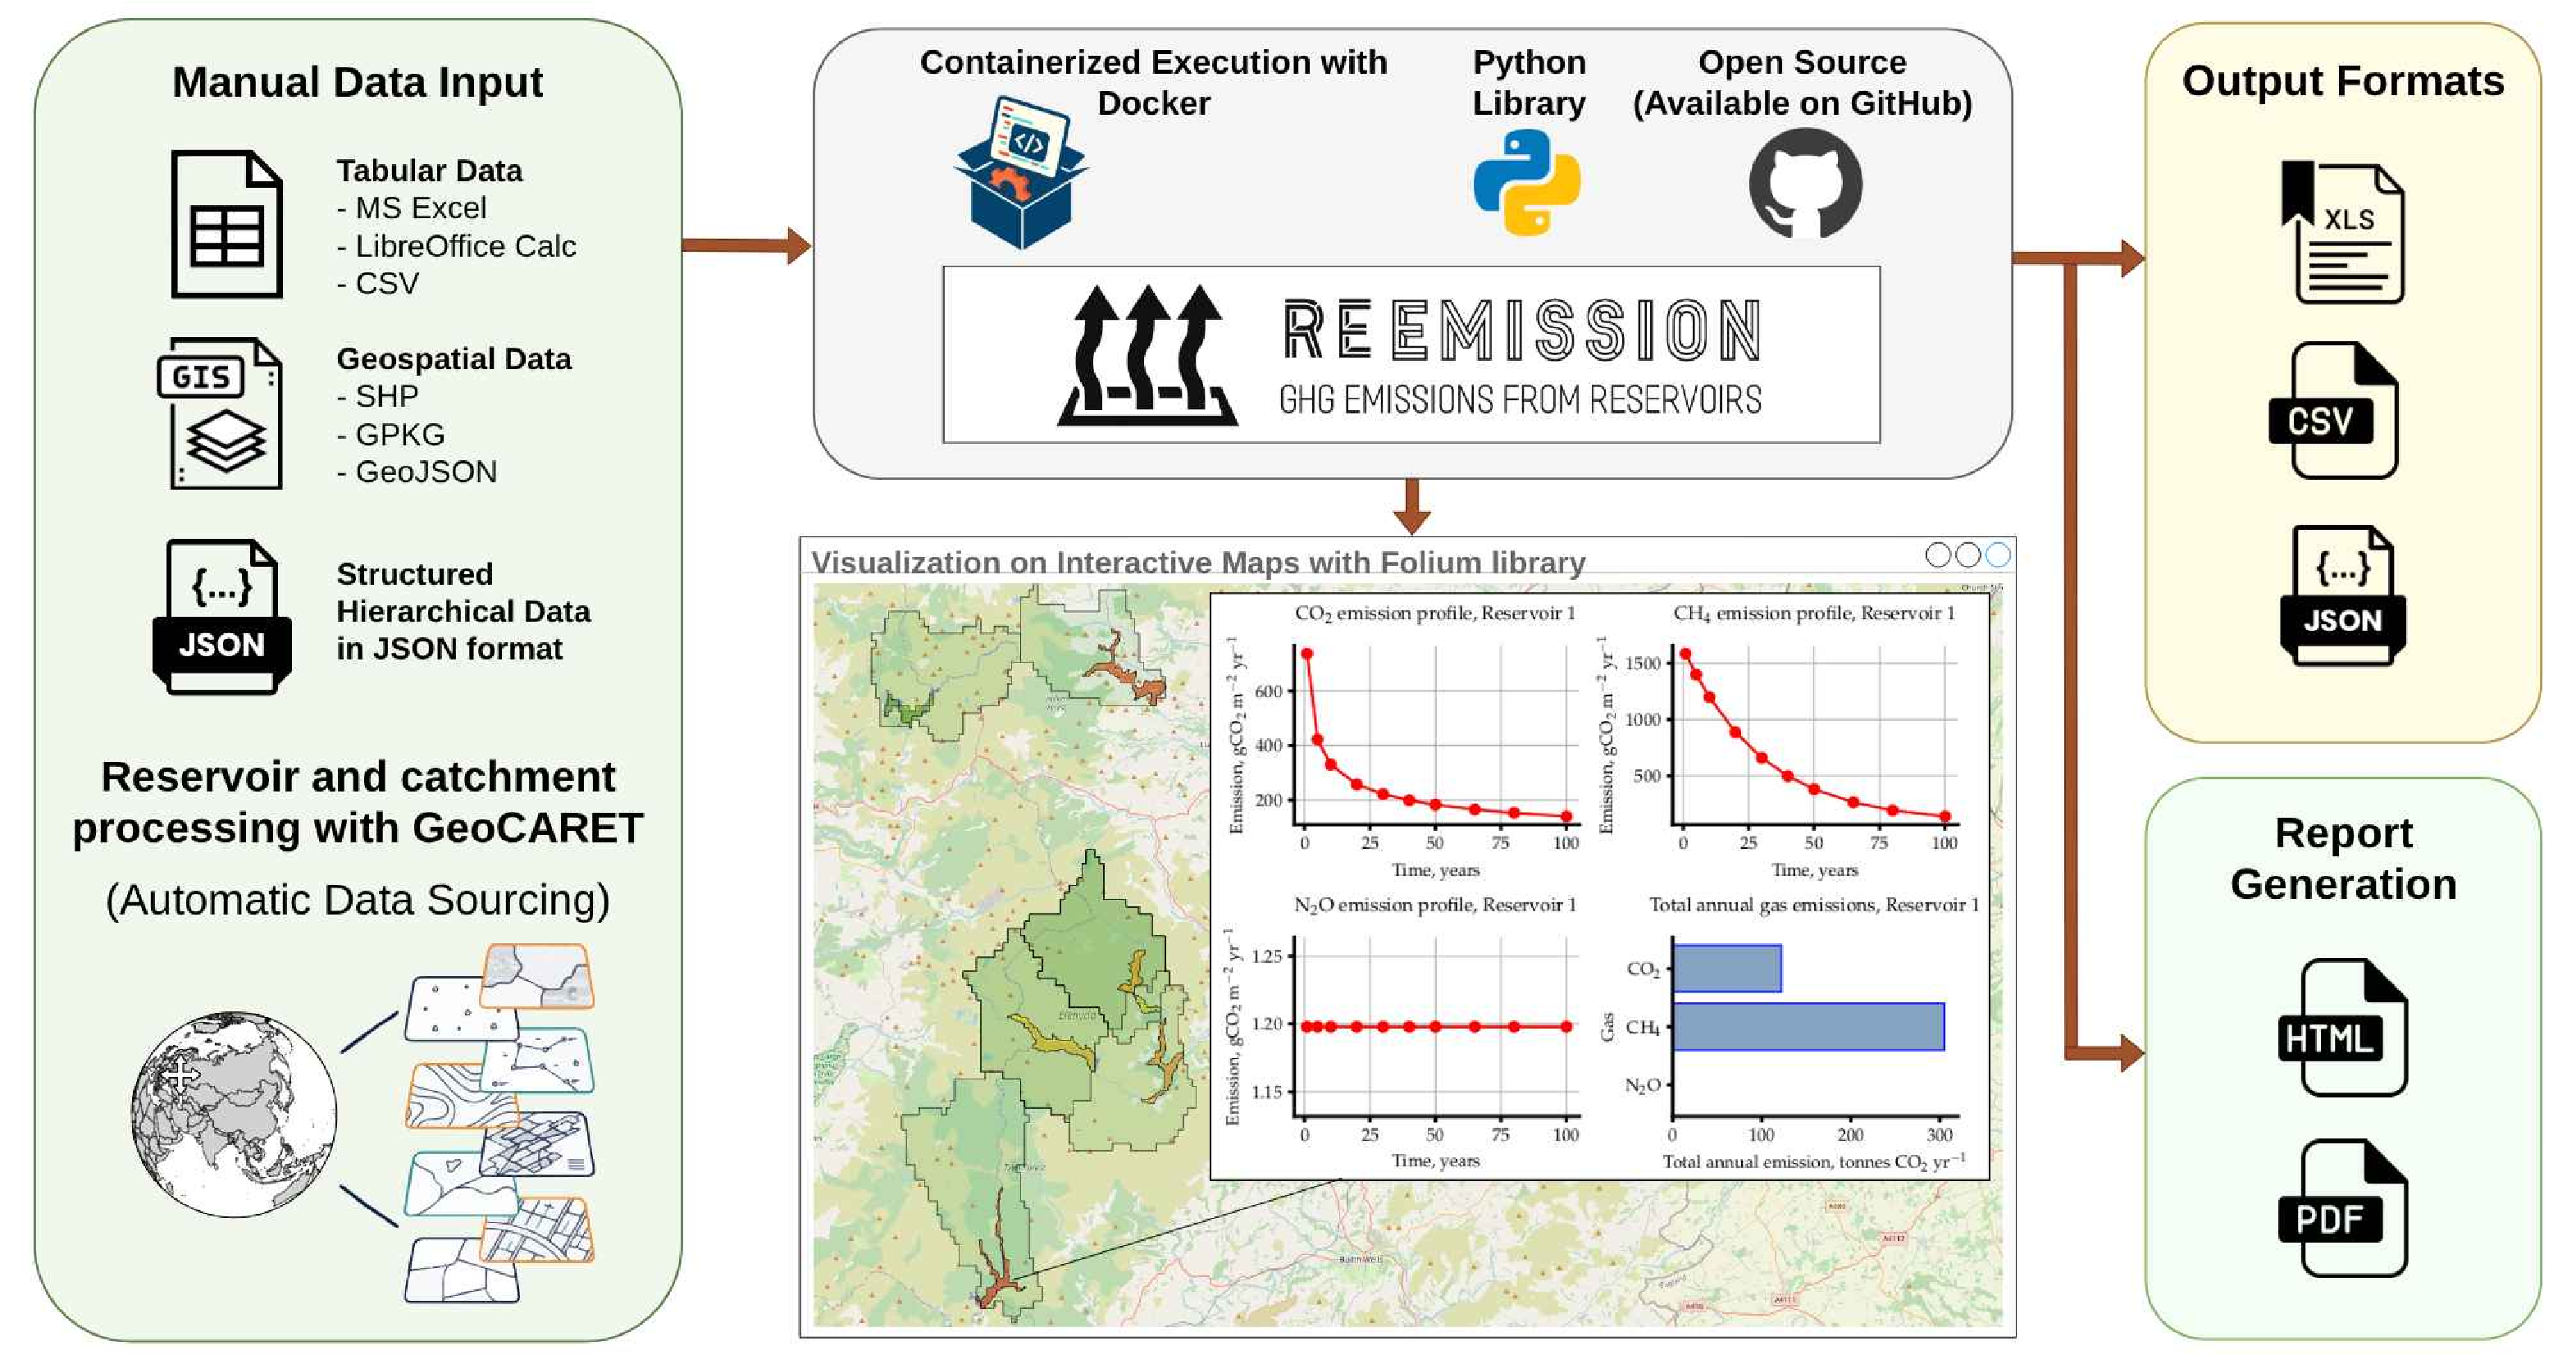
\includegraphics[width=1\textwidth]{figures/graphical_abstract_new_rev1.drawio_11zon.pdf}
\end{graphicalabstract}

%%Research highlights - OLD
%\begin{highlights}
%\item Command line tool and a Python library for calculating reservoir emissions.
%\item Configurable calculation and visualization options.
%\item Integrates with \acs{GIS}-based catchment and reservoir delineation tool.
 %%\item Automates emission calculations from multiple reservoirs.
%\item Supports multiple output and report formats.
%\item Applications in the United Kingdom and Myanmar highlight Re-Emission's features.
%\end{highlights}

\begin{highlights}
\item Re-Emission is a command-line tool and Python library for reservoir GHG analysis.
\item It automates GHG emission predictions across multiple reservoir systems.
%\item The tool offers configurable calculation and visualization of emission results.
\item It integrates with a GIS-based tool for reservoir and catchment analysis.
\item It supports multiple output and report formats and configuration options.
\item Case studies in the United Kingdom and Myanmar highlight Re-Emission's features.
\end{highlights}

%% Keywords
\begin{keyword}
automated emission assessments \sep reservoir emissions \sep modelling library \sep carbon footprint \sep limnology
%% keywords here, in the form: keyword \sep keyword
%% PACS codes here, in the form: \PACS code \sep code
%% MSC codes here, in the form: \MSC code \sep code
%% or \MSC[2008] code \sep code (2000 is the default)
\end{keyword}

\end{frontmatter}

\section{Introduction}
\label{sec:introduction}

Reservoirs are increasingly recognized as significant sources of biogenic \ac{GHG} emissions~\citep{Barros2011}, particularly in low-altitude tropical regions where emission intensities of hydroelectric dams (e.g., kg~CO$_{2e}$\,MWh$^{-1}$) may exceed those of fossil fuel power plants~\citep{Fearnside2002}. 
These emissions arise from the decomposition of organic matter that was either flooded during reservoir construction, transported into the reservoir by riverine runoff, or produced in situ through processes such as algal growth~\citep{Louis2000}.
Recent estimates suggest that existing reservoirs contribute approximately 5.2\% of global anthropogenic \ac{CH4} emissions and 0.2\% of \ac{CO2} emissions, together accounting for 1-2\% of total anthropogenic \ac{GHG} emissions~\citep{Soued2022}.
Continued and planned investments in new reservoir infrastructure are projected to exacerbate these emissions, hindering progress toward achieving the climate goals of the Paris Agreement.

With more than 3,700 new hydroelectric dams planned worldwide~\citep{Zarfl2015}, potentially contributing an additional 400\,MtCO$_{2e}$ per year~\citep{janus2025planning}, the sector’s total emissions are expected to rise markedly, even when accounting for uncertainties regarding which projects will be realized and their individual emissions.
Projections for planned reservoir investments in sectors such as flood control and water supply are less well documented but likely to be substantial, driven by efforts to enhance the resilience of water resources to climatic uncertainty~\citep{ipcc2018, Sarkodie2022}.
Given the potentially high areal \ac{GHG} fluxes from reservoirs, rigorous emission estimation is required both for planned reservoirs -- to inform low-carbon expansion strategies -- and for existing ones -- to improve the accuracy of global \ac{GHG} inventories and assess their climate impacts.
This highlights the need for practical, openly licensed tools that support routine emission estimation and foster continual development and broad uptake across the sector.

%Although several estimates of the total number and total area of reservoirs worldwide have been constructed, contemporary advances in remote sensing and global hydrological mapping have considerably increased our understanding of their true extent and distribution.
%\citet{Downing2006} estimated the number of impoundments globally at 515,149 with a total area of 258,570~km$^2$
%More recent studies provide significantly higher estimates: $\sim$2.8 million reservoirs with a total area of $\sim$530,000~km$^2$~\cite{Mulligan2020} and $\sim$2.5 million with $\sim$642,000~km$^2$ total surface area~\cite{LehnerMessager2023}. 
%All of the above figures are considerably larger than those reported in global dam databases such as \acs{FHReD}~\cite{Zarfl2015FHReD} ($\sim$40,000), \acs{GOOD2}~\cite{Mulligan2021GOOD2} ($\sim$38,667), or \acs{ICOLD}~\cite{ICOLD2020} ($\sim$58,700). 
%These discrepancies stem largely from improved satellite imagery and detection methods that can now identify millions of small and previously undocumented reservoirs.
%Given the likely exclusion of numerous existing reservoirs with unquantified atmospheric impacts, current global emission estimates may require reassessment to account for these new contributions.

Several studies have addressed the methodological challenges of quantifying reservoir emissions and have provided estimates of \ac{GHG} emissions from existing reservoirs at both global~\citep{Barros2011, Soued2022, Deemer2016, Prairie2018, Harrison2021} and regional scales~\citep{Hidrovo2017, Rasanen2018, Almeida2019, Hansen2022}. 
These studies have shown that reservoir emissions are shaped by a complex interplay of hydro-morphological, edaphic, climatic, and land-use characteristics of reservoirs and their catchments~\citep{Deemer2016, Prairie2021} requiring multi-variate emission models.
Meanwhile, current global assessments, including the most recent~\citep{Harrison2021, Soued2022}, have relied on empirical flux approximations derived from a limited number of measured sites, rather than on the direct application of spatially explicit emission models to individual reservoirs.
While these approaches have been instrumental in advancing our understanding of global reservoir emissions, they offer limited capacity to capture the variability in fluxes arising from site-specific environmental conditions and reservoir characteristics -- an aspect that remains crucial for informed reservoir planning~\citep{janus2025planning} and for further improvement of global emission estimates.
A major barrier to moving beyond Tier~1 \acfp{EF} and upscaling is the lack of software capable of applying spatially explicit emission models to estimate reservoir emissions at national, regional, and global scales.

%Moreover, s the measurement data used for upscaling are biased toward large, deep hydroelectric reservoirs~\citep{Hansen2022} and underrepresent smaller, shallower systems rich in organic matter that favour methane production~\citep{Malerba2022, WANG2025123441, SHI2025}, recent global \acp{EF}~\citep{Harrison2021, Soued2022} likely underestimate emissions from small reservoirs, such as those used for irrigation.

The most comprehensive and widely recognized model for estimating reservoir \ac{GHG} emissions is the G-res model~\citep{Prairie2017b, Prairie2021}, which provides spatially explicit estimates of both gross and net emissions by accounting for anthropogenic and natural sources, as well as a broad range of climatic, hydro-morphological, edaphic, and land-use drivers.
G-res is accessible via the publicly available web-based G-res Tool~\citep{prairie2017gres}. %, which offers free assessments for non-commercial users, while commercial applications require validation by the G-res team for a fixed fee.
Although the G-res Tool (v3.31) is easy to use, supported by a distinguished expert committee, and widely regarded as an industry standard, it is primarily designed for single-reservoir assessments.
It enables retrieval of selected input parameters from global geospatial datasets via Google Earth Engine~\citep{Gorelick2017}; however, because this process must be performed manually, its capability to support multi-reservoir analyses is currently limited.
Furthermore, as the tool is closed-source, it cannot be freely modified or extended by users, which constrains its adaptability for customized workflows and advanced applications, including stochastic modelling, strategic planning, and the integration of custom sub-models.

%The development of a free open-source alternative could offer the following benefits: (i) direct use of complete emission models, instead of upscaling methods, may help removing potential biases in global estimates and improve the accuracy of emission estimates for individual reservoirs, (ii) they will enable a more precise estimation of emissions from reservoirs whose characteristics fall outside the range of values represented in the measurement data sets (iii) they will enable an easier transition from Tier~1 may not be adequate to represent emission rates in different regions as well as different reservoir morphologies into more methodological methods without imposing significant overheads in terms of costs and time, (iv) 

%This upscaling approach assumes that areal fluxes for a given gas or emission pathway remain constant within a specific area of interest, such as a latitude~\cite{Harrison2021} or climatic zone~\cite{Soued2022} and does not take into account the effects of the multitude of emission drivers on emission rates~\citep{Deemer2016, Prairie2021} that vary widely across the diverse reservoir morphologies and their geographic settings.
%upscaling emissions from a small number of reservoirs with measured emissions to global emissions by 
%Precision due to identification of reservoir area and locations and estimation methods - ever growing numbers 
%However, these databases a rather high estimate for total area\,km$^2$ -- ~480,000 in GOOD2.
%Shows that missing data is for small reservoirs ...

Here, we introduce Re-Emission -- a free open-source Python library for estimating, visualizing, and reporting reservoir \ac{GHG} emissions. 
Re-Emission supports modifications and extensions, allowing users to incorporate new datasets, implement additional emission models or sub-models, adjust model parameters, and integrate project-specific requirements, thereby enabling fully customised reservoir-emission analyses.
Written in Python -- a widely used language in the scientific and engineering communities -- Re-Emission can be introduced into broader modelling or planning frameworks. 
Through its integration with the upstream reservoir and catchment processing tool GeoCARET~\citep{heettool}, it enables automated estimation of regional- to national-scale emission inventories using spatially explicit models, thus advancing beyond Tier~1 approximations in line with recommendations from the IPCC~\citep{IPCC2019}.
The G-res implementation within Re-Emission has been validated against the published G-res Tool~\citep{prairie2017gres, Prairie2021} (v3.31), ensuring that the software can be reliably used for practical assessments or reservoir \ac{GHG} emissions.

This paper is structured as follows.
First, we review the availability of software for reservoir emission modelling and position Re-Emission within this broader landscape.
Second, we provide a high-level overview of the software architecture, highlighting its main components and capabilities.
Third, we outline key features of the tool, including its dual use as a Python library for simulating reservoir emissions and as an implementation of existing models. 
We describe the basic usage of the Python library, available configuration options, supported input and output formats, and emission-reporting functionalities.
Fourth, we demonstrate an optional execution method via Docker and integration with GeoCARET~\citep{heettool} -- a command-line tool written in Python for delineating and analysing catchments and reservoirs using Google Earth Engine's cloud computing platform and assets~\citep{Gorelick2017}. 
Finally, we present two use cases that demonstrate the practical utility of Re-Emission in real-world settings, applying the framework to estimate emissions from roughly 250 reservoirs in Myanmar and the United Kingdom.


\section{Availability of software for reservoir emission modelling}
\label{subsec:software_and_code}

Despite growing research interest and practical relevance (see the historical review in the Supplementary Materials), software tools for modelling reservoir \ac{GHG} emissions remain limited.
Only a small number of modelling frameworks are accompanied by openly available tools that practitioners can readily apply.

Among currently available solutions, the G-res Tool~\citep{Prairie2017b,prairie2017gres} -- v3.31 at the time of writing -- constitutes the most advanced and operationally mature implementation currently accessible to practitioners.
It provides a web-based interface designed for hydropower developers, consultants, and stakeholders, implementing the G-res empirical regression model to estimate net anthropogenic \ac{GHG} emissions from reservoirs using widely available inputs without requiring field measurements~\citep{Prairie2021}. 
The tool supports allocation of emissions to reservoir services and includes modules to account for emissions associated with construction and infrastructure.
%Validation of tool results is required for public disclosure in commercial applications, which lends credibility and ensures appropriate use of the methodology.
The G-res Tool is available at no cost for non-commercial use, while commercial users are subject to a review and validation process by the G-res Team, incurring a fixed fee.
In addition, the G-res team offers further paid assessment services (e.g. ``Results Report'' and ``Full Report'' options) that provide certified emission estimates and detailed reporting ~\citep{prairie2017gres}.
The G-res Tool uses empirical, regression-based statistical models to estimate reservoir \ac{GHG} emissions.

Mechanistic (process-based) models such as CE-QUAL-W2~\citep{Berger2014}, LAKE~2.0~\citep{Lomov2024, Stepanenko2016}, and the \ac{EFDC} model~\citep{hamrick1992, SHI2025} are generally embedded within broader environmental or hydrodynamic modelling frameworks.
These models explicitly simulate the thermal and biogeochemical dynamics governing \ac{GHG} production and transport, offering higher process fidelity but reduced suitability for routine or large-scale assessments.
Their accessibility also varies: \ac{EFDC} is distributed as proprietary Windows executables without source code or official support, whereas LAKE~2.0, though open-source and cross-platform, is available only upon request rather than through a public repository.
By contrast, CE-QUAL-W2 is freely available under the MIT license and has been successfully applied in reservoir emission studies~\citep{Berger2014, Wu2022}.
Several other open-source lake models -- such as Flake, GLM, Simstrat, and MyLake -- are available and can be run individually or collectively via the LakeEnsemblR R package for ensemble lake modelling~\citep{Moore2021}.
These lake models can be extended with emission processes -- see, for example, \citep{Soued2020exp} -- but such implementations remain very limited.

The scarcity of free, open, extensible, and customizable software for reservoir \ac{GHG} emission assessment underscores a persistent gap between scientific model development and practical implementation.
Bridging this gap is essential to translate research advances into operational tools and to integrate emission models into broader frameworks for low-carbon reservoir planning and assessment -- many of which still rely on Tier~1 approaches~\citep{Almeida2019, Carlino2024, Tangi2024}.
Developing open-source, modular software ecosystems represents a crucial step toward enabling such integration.

\section{The Re-Emission package}
\label{sec:reemission}

Re-Emission is a free, open-source software package written in Python and supplied under the GNU General Public License v3.0, designed to be used both as a library and a \acf{CLI} tool. It serves two main purposes.

First, it provides an openly available and documented collection of Python classes that form a foundation for experimenting with existing reservoir emission models and developing new extensions.
The software is structured around the G-res framework, which offers a blueprint for estimating CO$_2$ and CH$_4$ emissions through multiple pathways and introduces the methodology for estimating emissions attributable solely to reservoir creation, i.e. ``What Does the Atmosphere See?''~\citep{Prairie2018}.
Following the G-res framework, Re-Emission reports gross and net emissions integrated over a 100-year horizon, along with emission trajectories showing their evolution over time from the impoundment year.
The hydro-morphological, edaphic, climatic, and land-use emission drivers are defined on catchment and reservoir levels and instantiated from input-data using respective \texttt{Catchment} and \texttt{Reservoir} classes.
By adopting the conceptual and structural design of G-res, Re-Emission enables researchers to extend the framework with new emission models and submodels without having to develop their own interfaces or reimplement existing formulations.

Second, Re-Emission provides a free and open-source implementation of the state-of-the-art G-res model~\citep{Prairie2021}, two reservoir phosphorus retention models~\citep{larsen1976, Maavara2015}, the nitrogen and phosphorus land export model of \citet{McDowell2020}, and two nitrous oxide emission models~\citep{Maavara2019, Akbarzadeh2019}.
Our software accurately reproduces the behaviour of the G-res Tool v3.31 -- the web-based interface implementation of the G-res model -- when using equivalent phosphorus retention and terrestrial export submodels (see Emission Model Validation and Supplementary Results).
The nitrous oxide emission models are currently unvalidated and considered experimental.
Model parameters can be configured via external configuration files or adjusted dynamically at runtime, supporting applications such as sensitivity analysis and calibration.
The implementation also supports batch processing of multiple reservoirs, and emission reporting and visualization in different formats.

Practical examples of implementing such capabilities are illustrated in a set of Jupyter Notebooks~\citep{Kluyver2016jupyter} and an accompanying demo (see \emph{Software Availability}).
Additional details on the software architecture and functionality are presented in the following sections.

\subsection{Design}
\label{subsec:design}

\begin{figure}[ht]
    \centering
    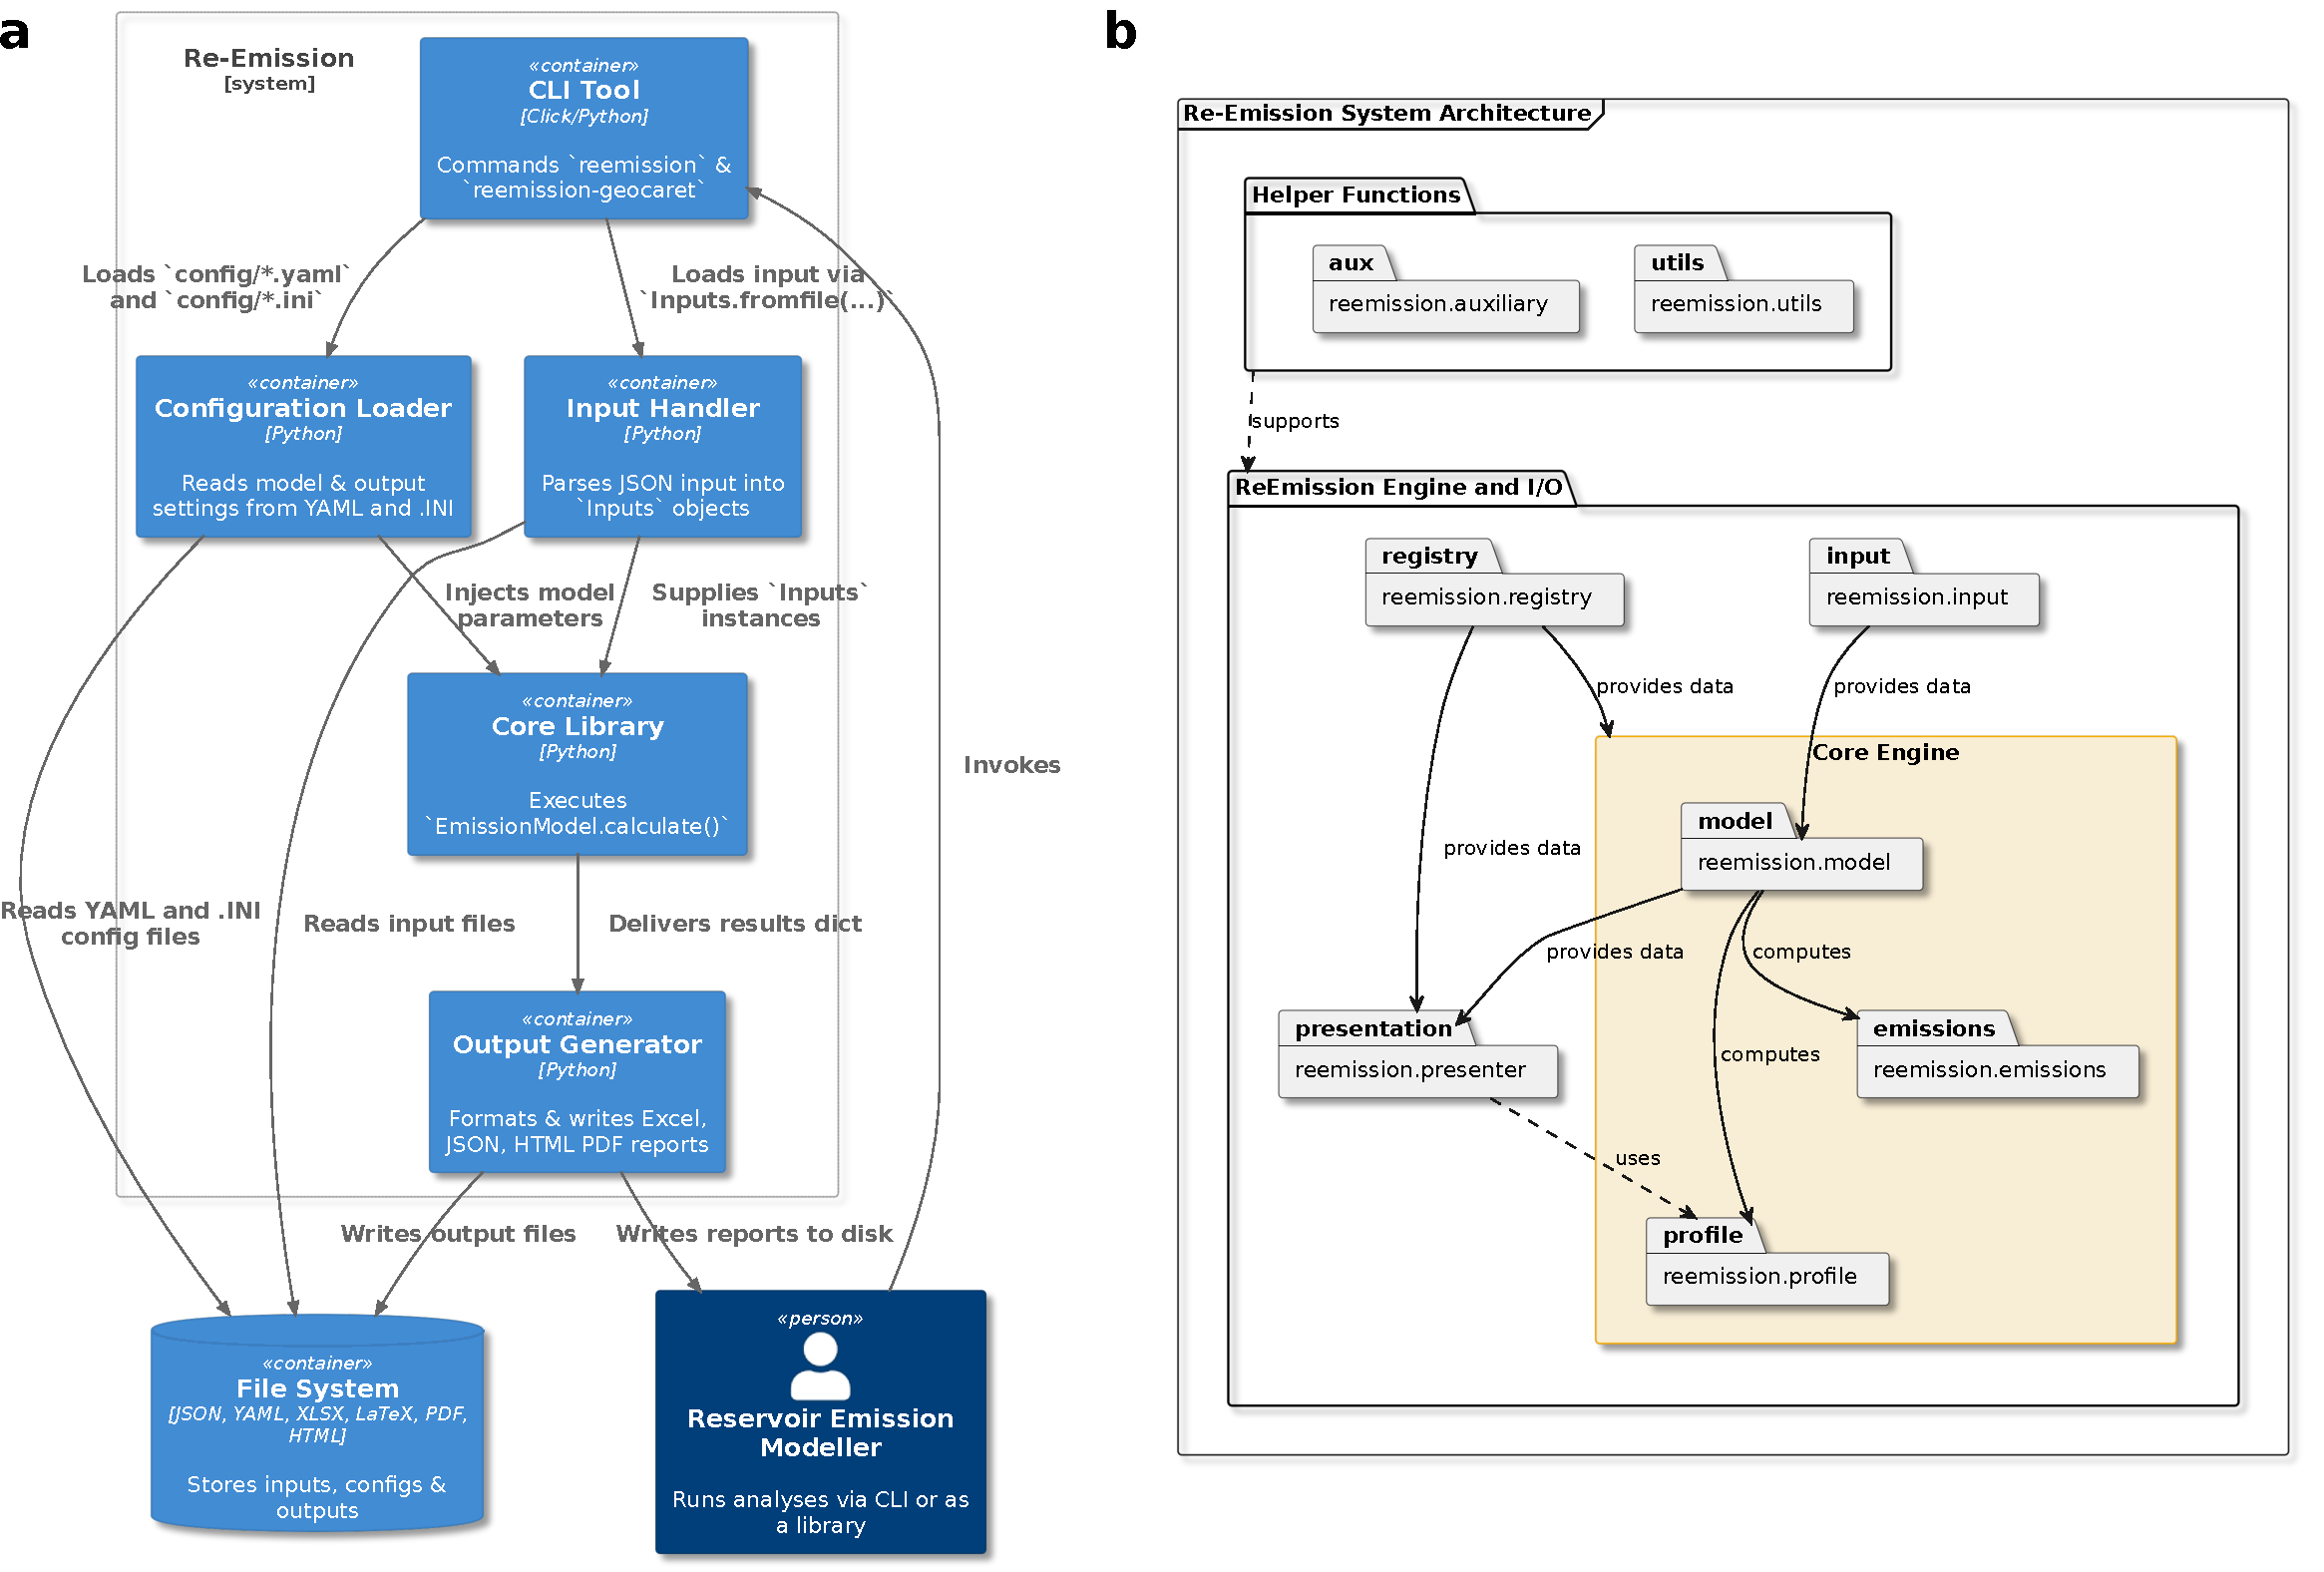
\includegraphics[width=0.99\textwidth]{figures/high_level_achitecture.pdf}
	\caption{Architecture of Re-Emission. \textbf{a}, Container-level interactions showing key components, their functionalities, and data flow between system elements. Users can interact with the \acf{CLI} or Python library to load configuration parameters and input data, run the core emission models, and generate reports in multiple formats (Excel, JSON, PDF, HTML). Configuration files specify model parameters and presentation settings for the outputs, while the file system manages input and output storage. \textbf{b}, Package dependency view highlighting the modular structure and inter-package relationships within the system.}
    \label{fig:high_level_archtecture}
\end{figure}

The high-level architecture of Re-Emission is illustrated in Figure~\ref{fig:high_level_archtecture}.
Re-Emission can be used either via a \acf{CLI} or by directly accessing its Core Library components within Python scripts, as shown in Figure~\figref[a]{fig:high_level_archtecture}.
\ac{CLI} serves as the primary user interface, enabling emission analyses through straightforward commands.
When a command is executed, control is passed to a configuration loader, which parses and validates the user-defined model parameters, execution settings (e.g., selection of submodels), and presentation options (e.g., choice of output variables and associated metadata).
Default configurations specified in YAML and INI files are located in the \vrbbrk{reemission/config/} directory.
Users can additionally override these settings by providing custom configuration files and including the path to the configuration folder in the command. 
The configuration settings are passed to both the Core Library and the \vrbbrk{reemission.presenter} module (Figure~\figref[b]{fig:high_level_archtecture}).
This design enforces a clear separation between logic (model equations) and data (parameters and inputs).

Input data are provided in JSON format and include reservoir, catchment, and climatic variables. 
These variables are read by \vrbbrk{reemission.input} and converted into a strongly typed \vrbbrk{Inputs} object used by the emission model.
Input data may be compiled manually from various data sources or generated automatically through upstream processing tools such as GeoCARET~\citep{heettool}, with which Re-Emission integrates (see Section~\ref{sec:integration}).
Upon completion of a model run, outputs are passed to a reporting engine, which generates results in multiple formats, including Excel workbooks (XLSX), structured JSON files, and HTML and PDF reports.
Presentation functionality is handled by \vrbbrk{reemission.presenter}, which collates inputs, outputs, and intermediate variables from \vrbbrk{reemission.model} and \vrbbrk{reemission.profile}, enabling both textual and graphical visualisations of the simulation outputs.
The loading, modification, and reuse of configuration files are managed by the \vrbbrk{reemission.registry} module.
%e cumulative reservoir emissions over time, based on each reservoirs' impoundment dates and their respective emission decay rates. 
% % -- such as regression coefficients, pre-impoundment emissions, and nutrient exports from land -- such as choice of submodels
%The input data and configuration settings are then routed into the Core Library highlighted in Figure~\figref[b]{fig:high_level_archtecture} by a lemon yellow rectangle. 
%The Core Library comprises the emission model, which runs the analysis using selected emission models and passes the results to \vrbbrk{reemission.presenter}. 

\begin{figure}[ht]
    \centering
    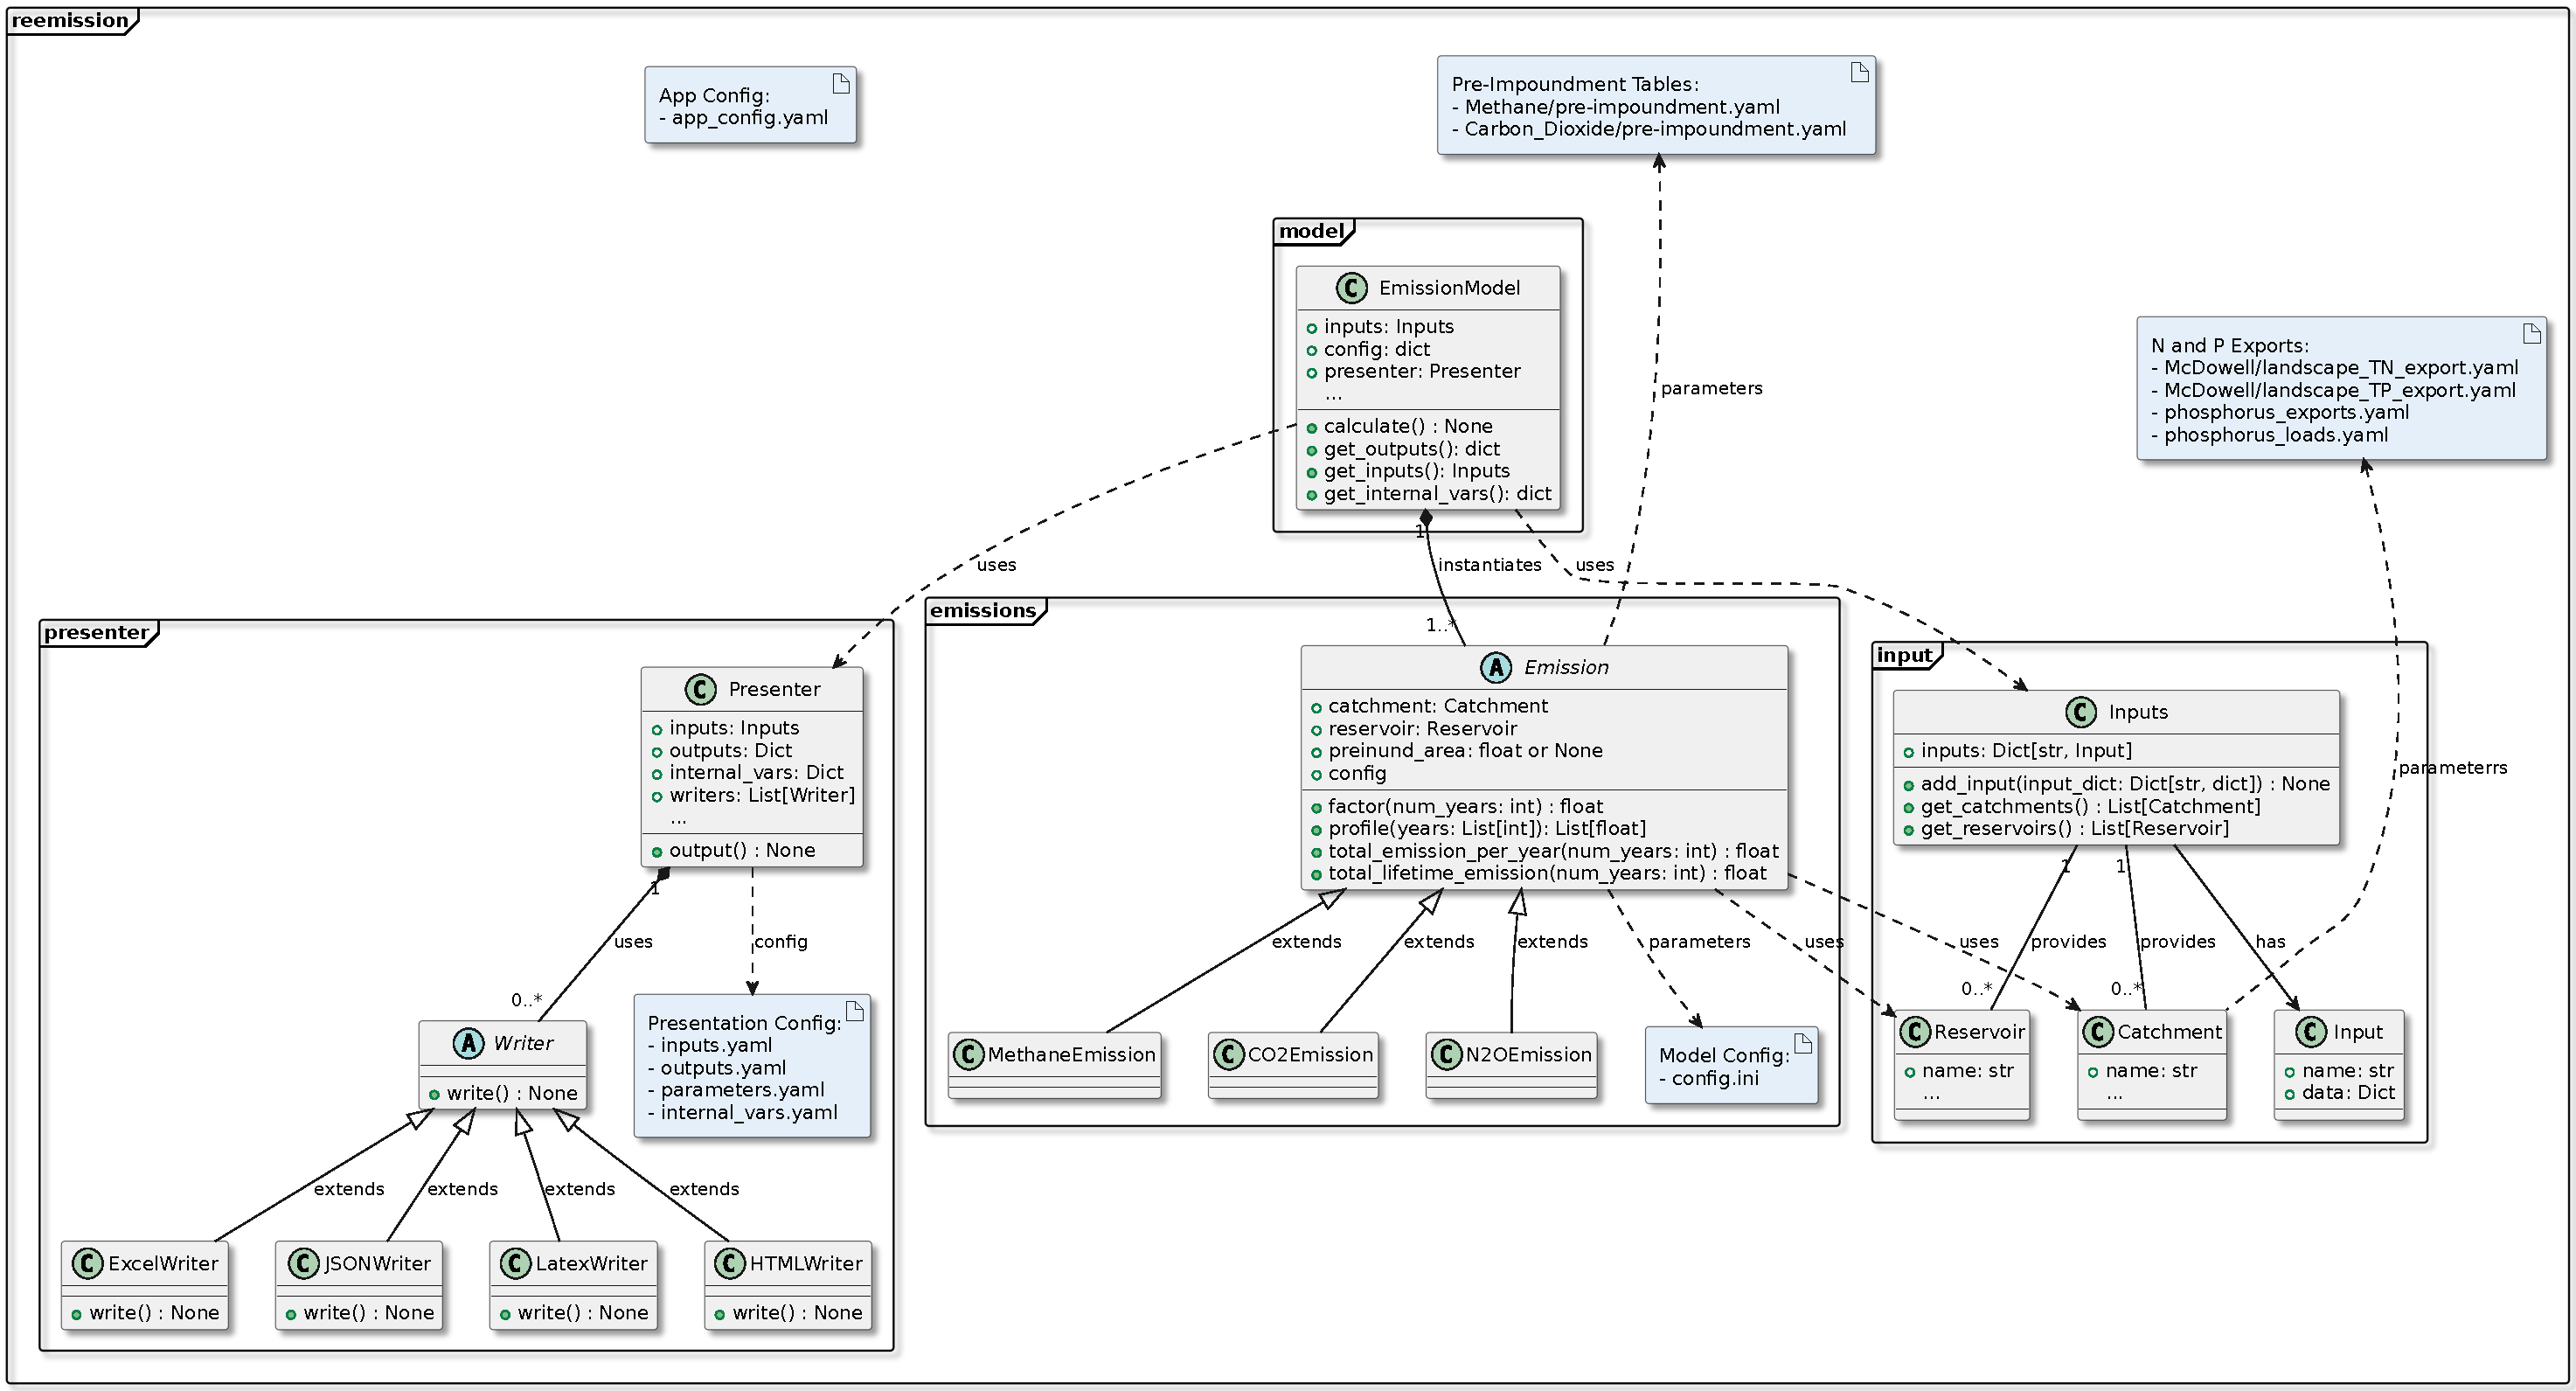
\includegraphics[width=0.99\textwidth]{figures/high_level_uml2.pdf}
	\caption{UML class diagram of Re-Emission, illustrating key classes and their relationships. Core components include \texttt{EmissionModel}, \texttt{Reservoir}, \texttt{Catchment}, \texttt{Emission}, \texttt{Inputs}, and \texttt{Presenter}, with abstract interfaces used to enforce modularity and extensibility.}
    \label{fig:high_level_uml}
\end{figure}

A more detailed view of the internal structure and inter-class relationships is shown in the UML class diagram in Figure~\ref{fig:high_level_uml}.
The \texttt{EmissionModel} class encapsulates the core simulation logic, including the instantiation of \vrbbrk{Reservoir}, \vrbbrk{Catchment}, and \vrbbrk{Emission} objects (e.g., \vrbbrk{MethaneEmission} for CH$_4$), and the subsequent computation of intermediate and final output variables.
The \vrbbrk{Reservoir} and \vrbbrk{Catchment} instances are introduced to the \vrbbrk{EmissionModel} object via the \vrbbrk{Inputs} class.
Each \vrbbrk{Emission} object inherits from an abstract \vrbbrk{Emission} base class that defines four abstract methods that must be implemented by all subclasses.
The \vrbbrk{Presenter} class relies on \vrbbrk{Writer} objects to export outputs in different formats.
All \vrbbrk{Writer} implementations inherit from an abstract \vrbbrk{Writer} base class that defines a unified a unified interface for output generation.
Supported output formats include JSON, XLSX, PDF (via \LaTeX), and HTML.
The \vrbbrk{Reservoir}, \vrbbrk{Catchment}, \vrbbrk{Emission}, and \vrbbrk{Presenter} classes are parametrized through configuration files that specify regression coefficients, pre-impoundment emission factors, nutrient export rates, and presentation settings.
Further details on the internal structure of the \vrbbrk{Reservoir} and \vrbbrk{Catchment} classes, along with the representation of input data, are provided in the Appendix in Figure~\ref{fig:river_network_emissions_uml}.

\subsection{Using Re-Emission as a library}
\label{subsec:scripting}

Emission calculations can be performed step by step: first by constructing \vrbbrk{Reservoir} and \vrbbrk{Catchment} instances, and then instantiating and running individual \vrbbrk{Emission} objects (for CO$_2$, CH$_4$, etc.), as shown in Listings~\ref{lst:em_calc_setup} and~\ref{lst:em_calc} in the Appendix.
Alternatively, the \vrbbrk{EmissionModel} class provides a streamlined interface for the same process, (see Listing~\ref{lst:em_calc_file}).
In addition to simplifying model execution, \vrbbrk{EmissionModel} class enables exporting results in multiple formats via the \vrbbrk{Presenter} class (see Listing~\ref{lst:em_calc_presentation}).
In both usage modes, the analytical workflow -- excluding result presentation -- follows the algorithmic structure in Algorithm~\ref{alg:reemission}.
Input data and model parameters are read from JSON input fles and configuration files (INI and YAML), and validated prior to computation.
Emissions are then calculated for each reservoir defined in the dataset, and raw results are saved to a JSON output file.

\begin{algorithm}[H]
\caption{Reservoir Emission Estimation}
\label{alg:reemission}
\SetKwInOut{Input}{Input}
\SetKwInOut{Output}{Output}

\AlgoDisplayBlockMarkers

\Input{Input file path (e.g., \texttt{input\_file.json})\\
       Configuration file path (e.g., \texttt{config\_file.yaml})}
\Output{Output file path (e.g., \texttt{output\_file.json})}

\BlankLine
Load input data from \texttt{input\_file.json}\;
\If{input is invalid}{
    Raise error and exit\;
}
Initialize model parameters from configuration file\;
\ForEach{entry in dataset}{
    Instantiate \texttt{Reservoir} and \texttt{Catchment} objects\;
    Instantiate \texttt{CarbonDioxideEmission} and \texttt{MethaneEmission} objects\;
    Estimate annual CO\textsubscript{2} and CH\textsubscript{4} fluxes and flux profiles\;
}
Save results to \texttt{output\_file.json}\;
\end{algorithm}


\subsection{Command-Line Interface}
\label{subsec:cli}

Full \acf{CLI} usage instructions can be accessed by running \vrbbrk{reemission --help} in a terminal.
A typical command-line invocation is shown in Listing~\ref{lst:em_calc_cli}.
The input data are provided in \vrbbrk{input.json} and the outputs are generated in several formats, including PDF, JSON, XLSX, and HTML.
In addition to emission calculation, the \ac{CLI} offers commands for converting and modifying input datasets.
These features are discussed further in Section~\ref{sec:integration}, which focuses on integration with upstream reservoir and catchment data-processing workflows (see also Listing~\ref{lst:integration_cli}).

\begin{minipage}{0.95\textwidth}
\begin{lstlisting}[language=bash, label={lst:em_calc_cli}, caption={Re-Emission \ac{CLI}: Emission calculations using input.json as the source of input data.}]
> reemission calculate 
    input.json
    -o output.pdf -o output.json -o output.xlsx  -o output.html
    --author "John Smith" 
    --title  "Reservoir Emissions Analysis"
\end{lstlisting}
\end{minipage}

\subsection{Input and output data formats}
\label{subsec:input_output_formats}

The structure of the input and output data is shown in Figures~\ref{fig:input_data_format} and~\ref{fig:output_data_format}, respectively.
The input format is fixed and determined by the parameter requirements of the \vrbbrk{Reservoir} and \vrbbrk{Catchment} classes.
In contrast, the structure of the output data is user-configurable through YAML configuration files.
For clarity, the figures present only a representative subset of the full input and output content.
Where data have been truncated, omissions are indicated using bold, light-blue text followed by an ellipsis (...).

\begin{figure}[ht]
    \centering
    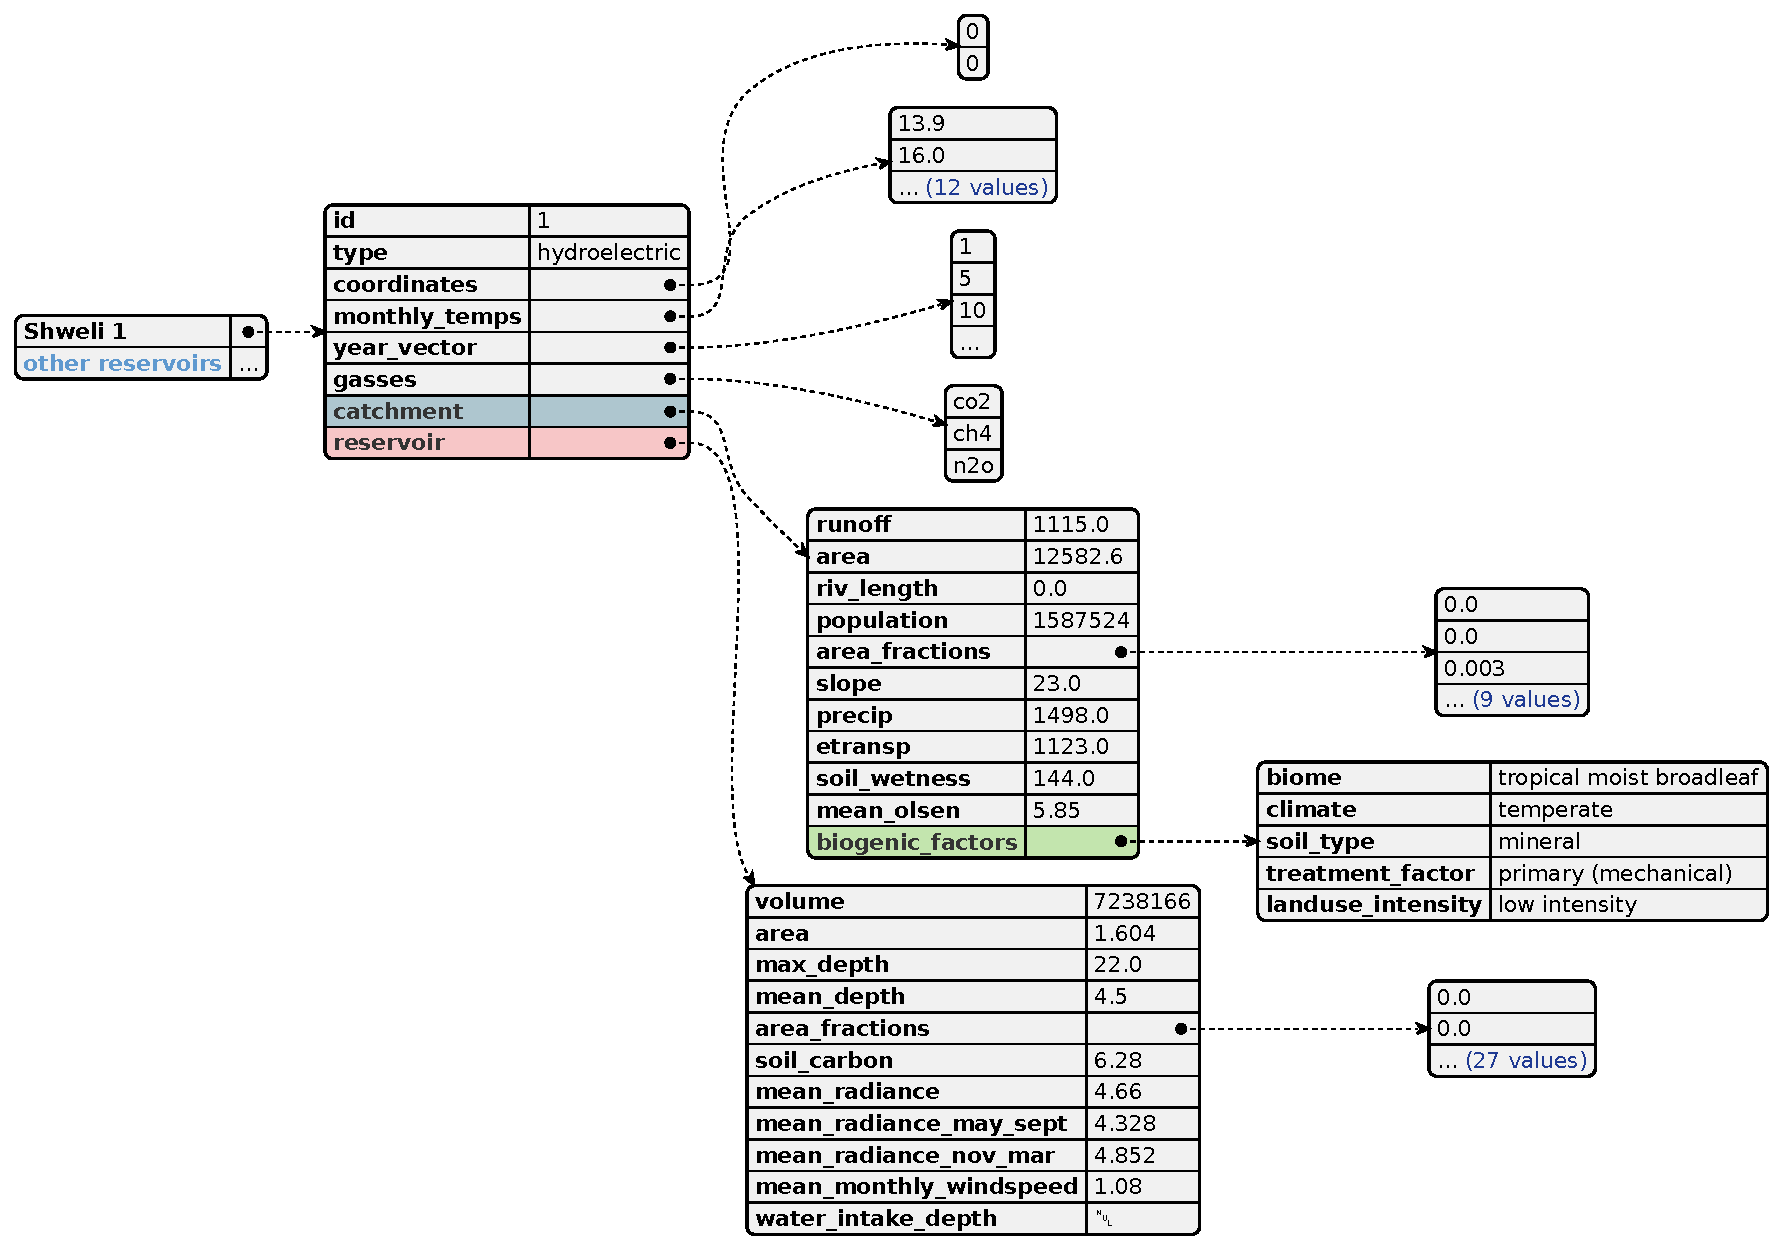
\includegraphics[width=0.75\textwidth]{figures/input_data_json.pdf}
    \caption{Structure of an input JSON file containing example data for a single reservoir. Entries related to catchment and reservoir parameters -- highlighted in steel blue and salmon, respectively -- correspond directly to fields defined in the \vrbbrk{Catchment} and \vrbbrk{Reservoir} classes. Selected values have been truncated for readability, with omissions indicated using light blue font colour followed by an ellipsis.}
    \label{fig:input_data_format}
\end{figure}

\begin{figure}[ht]
    \centering
    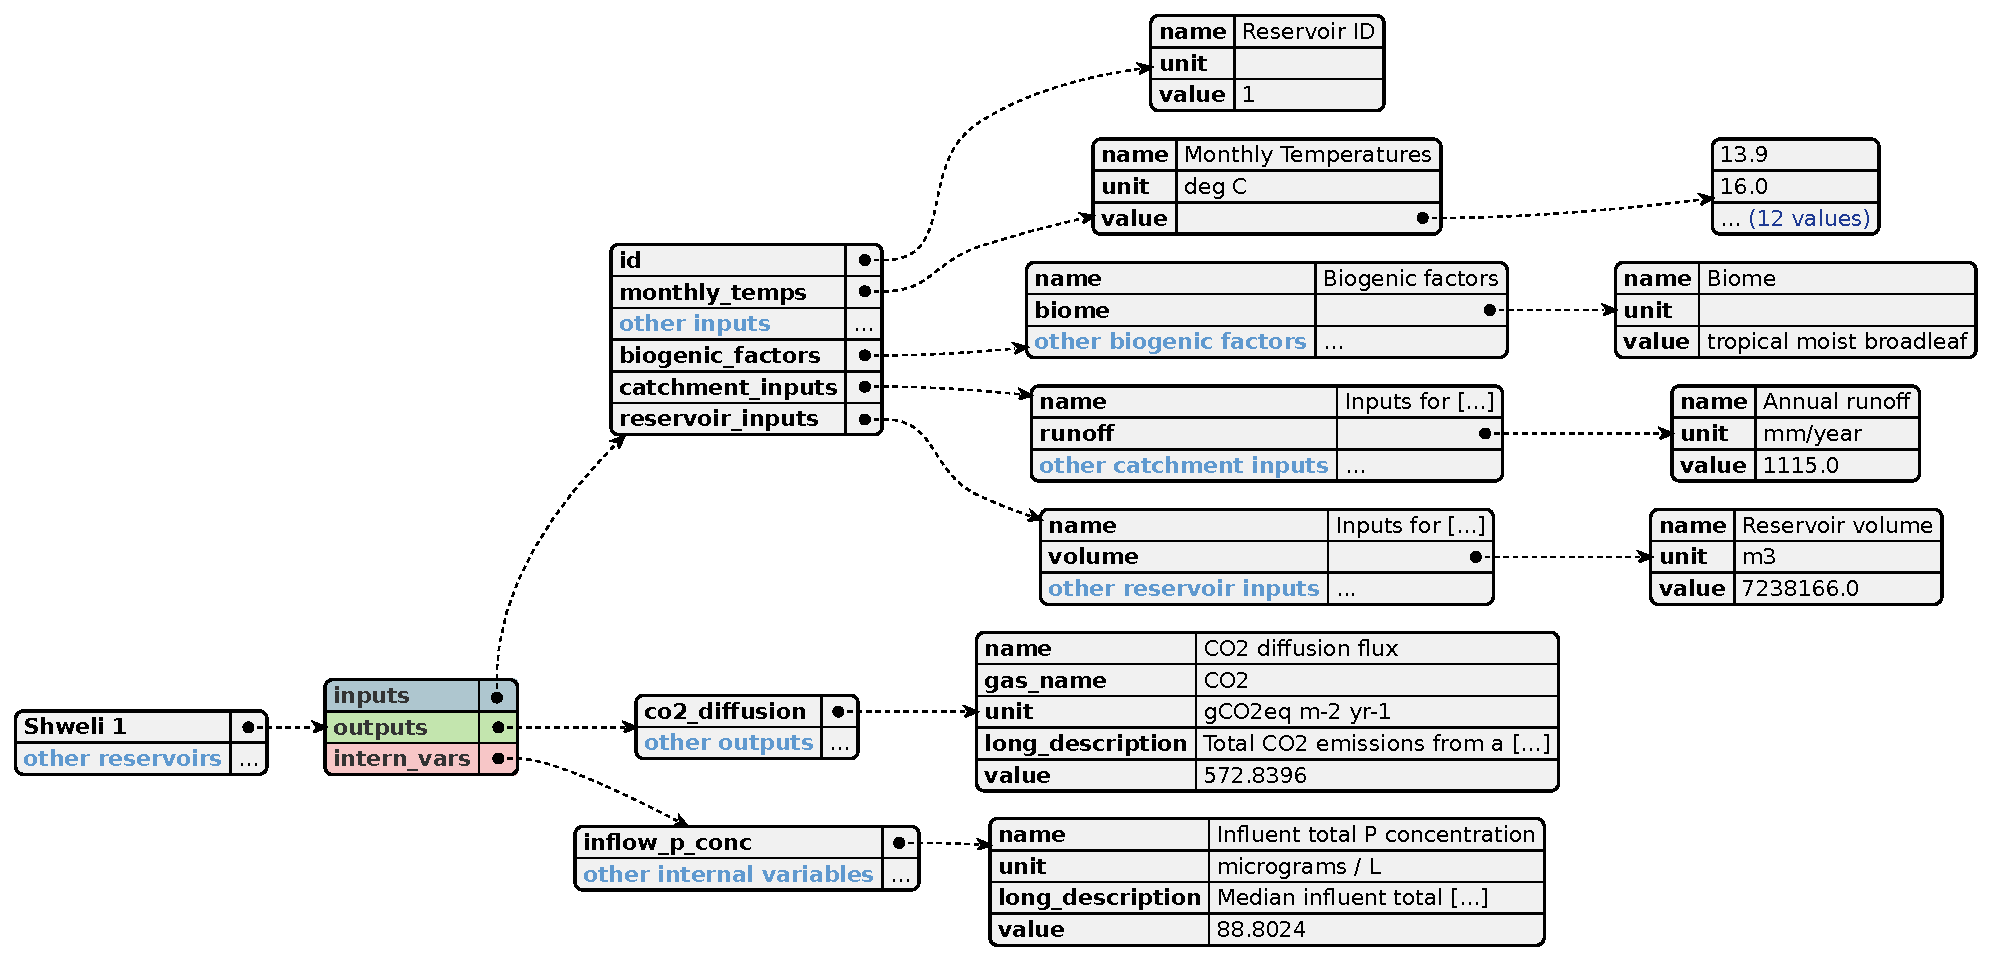
\includegraphics[width=0.9\textwidth]{figures/output_data_json.pdf}
    \caption{Structure of an example configurable output JSON file. The file is organized into three sections -- inputs, outputs, and internal variables -- highlighted in steel blue, olive green, and salmon, respectively. As the number of output entries can be arbitrarily large, selected values have been truncated for readability. Truncated content is indicated using light blue font colour followed by an ellipsis.}
    \label{fig:output_data_format}
\end{figure}

\subsection{Configuration options}
\label{subsec:config_options}

Configuration data -- including model parameters, options for the \vrbbrk{Presenter} class, and tabular inputs such as pre-impoundment emission factors or nutrient export coefficients -- is stored in INI and YAML files. 
The structure of the configuration files is illustrated in Figure~\ref{fig:config_uml} for presentation and model settings, Figure~\ref{fig:preimpoundment} for pre-impoundment emission factors, and Figure~\ref{fig:tp_tn_exports} for nutrient-export model parameterization..

Configuration files are registered and loaded lazily upon first access by the \vrbbrk{ConfigLoader} class.
The class also supports overriding default settings with user-defined configurations.
Instance of \vrbbrk{ConfigLoader} with registered configuration files is made globally accessible through the \vrbbrk{reemission.registry} module.

\subsection{Containerized execution using Docker}
\label{subsec:docker}

To ensure reproducibility and simplify the deployment of Re-Emission, we implemented a fully containerized workflow using Docker~\citep{merkel2014docker}, GitHub Actions, and the \acf{GHCR}, as illustrated in Figure~\ref{fig:docker_containerizing}.
This approach ensures consistent runtime behaviour across computing environments and eliminates the need for complex setup procedures, thereby lowering the technical barrier to adoption.

Docker is an open-source platform that packages applications and their dependencies into standardized units called containers, which run in isolated environments.
Re-Emission, together with the Python interpreter, essential libraries, and other dependencies, is encapsulated in a Docker image.
The source code and Docker configuration files (e.g., \verb|compose.yaml|) are maintained in a GitHub repository, with \ac{CI} managed via GitHub Actions. Whenever changes are pushed to the \verb|release| branch, a Docker image is automatically built and published to the GitHub Container Registry.
This image can be retrieved using the standard \verb|docker pull| command, assuming Docker is installed on the user’s system.

The Re-Emission \ac{CLI} can be executed via \verb|docker compose run reemission| from a directory containing the appropriate \verb|compose.yaml| configuration file.
This file is required at runtime to map directories between the container and the host system, enabling access to input files and writing of output results.
To further streamline Dockerized execution, a companion repository provides the necessary folder structure, configuration files, and volume mappings for running the Re-Emission container~\citep{janus_geocaret_reemission}; see Software Availability.

Currently, the shared Docker images for Re-Emission do not include a \LaTeX\ distribution, which is required for generating PDF reports via the \verb|pylatex| library.
This omission is deliberate: bundling a full \LaTeX\ system—such as TeXLive—would significantly increase the image size, reducing portability and practicality for lightweight deployments.
As a result, PDF report generation is not supported in the standard containerized version of Re-Emission.
Equivalent HTML-based reports can, however, be generated as described in Section~\ref{subsec:input_output_formats}.
Users requiring PDF report generation within Docker must build a custom image by extending the official Re-Emission image with a \LaTeX\ installation.
This can be accomplished by creating a new Dockerfile (see Listing~\ref{lst:docker_with_latex}) and building the image with the command:
\verb|docker build -t reemission-with-latex .| executed in the directory containing the Dockerfile.

\begin{figure}[ht]
    \centering
    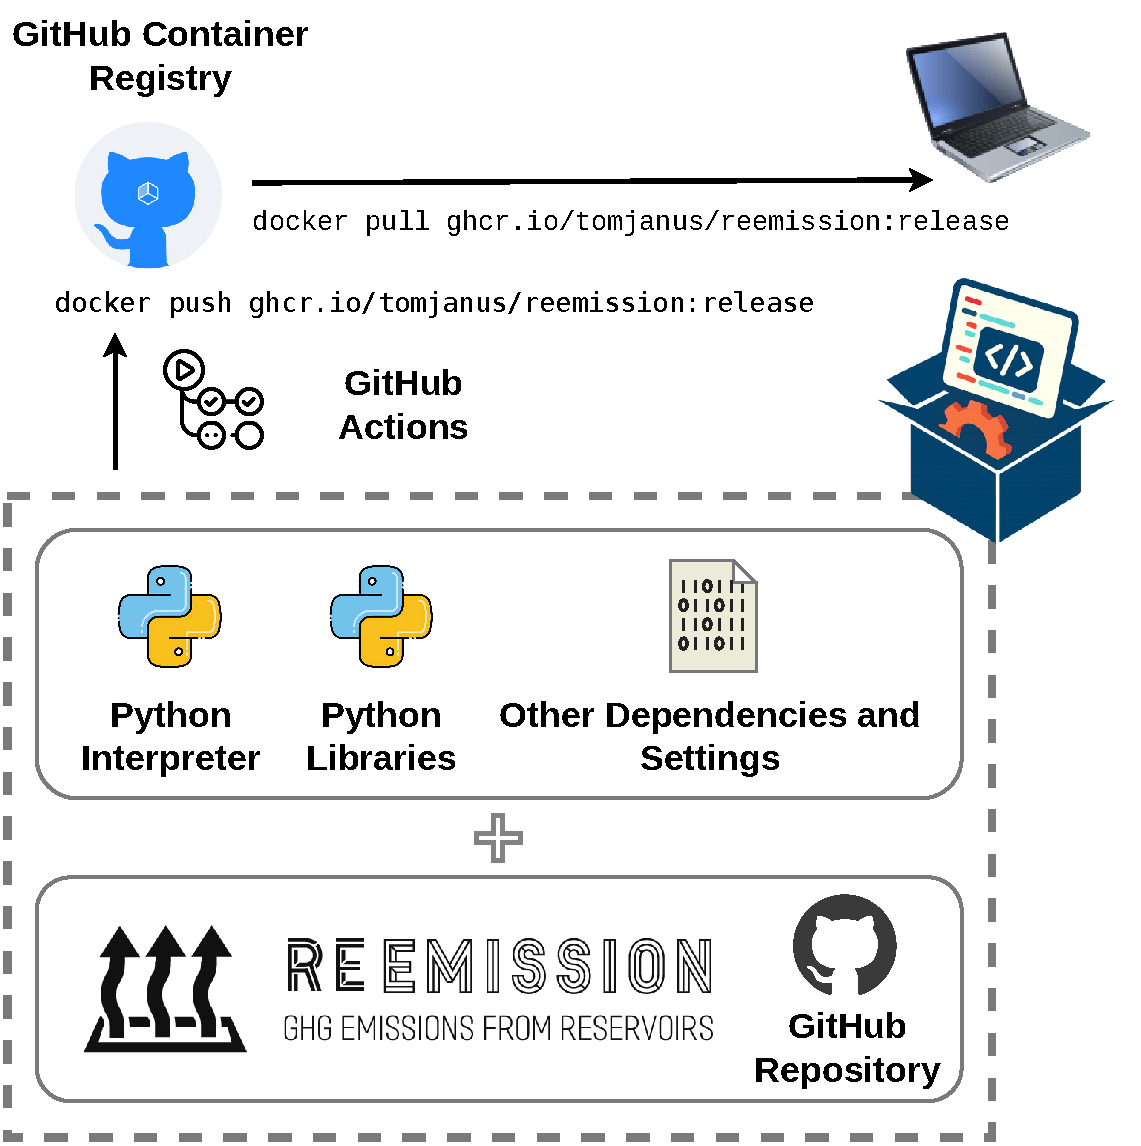
\includegraphics[width=0.55\textwidth]{figures/docker-explanation.drawio.pdf}
    \caption{{Containerized deployment of Re-Emission using Docker, GitHub Actions, and the GitHub Container Registry.}}
    \label{fig:docker_containerizing}
\end{figure}

\begin{minipage}{0.95\textwidth}
\begin{lstlisting}[language=Dockerfile, , label={lst:docker_with_latex}, caption={Dockerfile for extending the Re-Emission image with a full TeX Live installation to support PDF report generation via PyLaTeX.}]
# Dockerfile
FROM ghcr.io/tomjanus/reemission:release
# Install TeX Live
RUN apt-get update && \
    apt-get install -y texlive-full && \
    apt-get clean && \
    rm -rf /var/lib/apt/lists/*
\end{lstlisting}
\end{minipage}

\section{Integration with upstream reservoir and catchment processing}
\label{sec:integration}

Estimating emissions from multiple reservoirs using spatially explicit models such as G-res is challenging due to the effort required to source and derive input data.
When input variables are unavailable, they must be extracted from geospatial datasets using \ac{GIS} methods, typically involving delineation of each reservoir and its catchment, followed by processing diverse datasets such as \acp{DEM}, land cover maps, soil and biome classifications, and various climate-related datasets.
These steps are time-consuming, particularly at larger spatial scales.

To simplify this process, we provide functionality for generating input JSON files for Re-Emission from the outputs of the open-source Geospatial CAtchment and REservoir analysis Tool (GeoCARET)~\citep{heettool}.
GeoCARET implements algorithms for the statistical and geometric operations required to derive reservoir and catchment characteristics and executes them on \ac{GEE}~\citep{Gorelick2017} via its Python API.
This enables automated data acquisition and preprocessing across multiple reservoir sites, producing the inputs needed for the G-res model.
Although still under development, GeoCARET successfully generated input data for the two case studies presented here and for a recent study on hydropower planning with emission models~\citep{janus2025planning}.

Integration between the tools is provided via a suite of \ac{CLI} functions, illustrated in Listing~\ref{lst:integration_cli}, which:
(i) merge multiple tabular files and populate missing variables; (ii) convert tabular data to JSON format; and (iii) optionally merge individual reservoir and catchment shapefiles for mapping and visualization of emissions.
The workflow is further streamlined by running both tools within their Docker containers, coordinated through the Re-Emission-GeoCARET companion repository~\citep{janus_geocaret_reemission} (see \emph{Software Availability}).

Since GeoCARET relies on \ac{GEE}, which operates on Google Cloud and is not free for commercial users (although both services can be used free of charge with certain limitations for non-profit and research purposes), using Re-Emission together with GeoCARET for commercial applications may incur costs and may require a paid Google subscription.
A rough estimate of the cost of generating input data for an average reservoir for commercial purposes, along with a high-level overview of Google's usage plans for both commercial and non-commercial users, is provided in the Supplementary Materials.


\begin{minipage}{0.95\textwidth}
\begin{lstlisting}[language=bash, 
label={lst:integration_cli}, caption={Re-Emission CLI: Processing outputs from the GeoCARET reservoir and catchment processing tool.}]
# Step 1: Processing tabular GeoCARET outputs in multiple .csv files 
> reemission-geocaret process-tab-outputs \
    -i  geocaret_outputs.csv \
    -o  reemission_inputs.csv \
    -cv 'c_treatment_factor' 'primary (mechanical)' \
    -cv 'c_landuse_intensity' 'low intensity' \
    -cv 'type' 'potable'
# Step 2: Creating Re-Emission input JSON file from the tabular CSV data
> reemission-geocaret tab-to-json 
    -i reemisison_inptus.csv 
    -o reemission_inputs.json
# Step 3: Merging shape files (one per individual reservoir, catchment, dam, etc.) into combined shapes per geometry type
> reemission-geocaret join-shapes \
    -i  input_folder
    -o  output_folder
    -gp 'R_*.shp, C_*.shp, PS_*.shp'
    -f  'reservoirs.shp, catchments.shp, dams.shp'
\end{lstlisting}
\end{minipage}

%% Use \subsubsection, \paragraph, \subparagraph commands to 
%% start 3rd, 4th and 5th level sections.
%% Refer following link for more details.
%% https://en.wikibooks.org/wiki/LaTeX/Document_Structure#Sectioning_commands

%% Refer following link for more details.
%% https://en.wikibooks.org/wiki/LaTeX/Floats,_Figures_and_Captions
%% https://en.wikibooks.org/wiki/LaTeX/Importing_Graphics#Importing_external_graphics

\section{Materials and Methods}
\label{sec:materials_and_methods}

A detailed description of the materials and methods used to validate the Re-Emission's G-res model implementation against the results of the G-res Tool (v3.31) and our own R-based implementation, as well as to conduct both case studies -- estimating emission trajectories from existing and future reservoirs in Myanmar and performing parametric uncertainty analysis of diffusive CO$_2$ and CH$_4$ emission pathways -- is provided in the following subsections.

\subsection{Model validation}
\label{subsec:model_validation_methods}

To validate the implementation of the G-res model in Re-Emission, we independently re-implemented the model in the R programming language.
Both versions were then used to compute key outputs: gross and net areal CO$_2$ and CH$_4$ emissions across all modelled pathways together with the intermediate diagnostic variables involved in the emission calculations.
Via systematic cross-comparison of outputs, combined with a detailed review of both codebases, we minimised the likelihood of algorithmic or implementation-level discrepancies in Re-Emission.

To evaluate model fidelity across a wide range of input conditions, we generated a synthetic validation dataset by randomly perturbing categorical attributes from real reservoir records.
This approach allowed us to explore combinations of parameters that do not occur in the empirical data but are nevertheless plausible within the modelling framework.
The final dataset comprised 246 synthetic reservoirs derived from systems located in Myanmar and the United Kingdom.
Each synthetic entry was produced by randomly modifying key categorical variables -- land-cover classes, biomes, climatic regimes, soil types, land-use intensities, and catchment-scale wastewater treatment characteristics.

In addition, four real reservoirs from Myanmar and the United Kingdom were selected for direct comparison with the G-res Tool v3.31 web interface.
For each system, emissions were estimated using both Re-Emission and the official tool to provide an additional layer of verification and to ensure agreement with the current G-res Tool implementation.

\subsection{Calculation of emission trajectories (Myanmar)}
\label{subsec:myanmar_case_study_methods}

Information on existing and planned reservoirs in Myanmar -- including their locations, physical characteristics, and, where available, impoundment years -- was compiled from a range of databases and reports~\citep{ifc_dam_db, EA_Myanmar, Emmerton2015, opendevelopmentmya2018, PowerSector_Myanmar, sea2018}.
Emissions for each reservoir were estimated using Re-Emission, with input data derived from global open datasets using GeoCARET, following the methodology described in \citet{janus2025planning}.

Missing impoundment years were reconstructed using a hybrid stochastic procedure.
For irrigation reservoirs, known impoundment years were used to estimate the probability density of historical development via kernel density estimation (\acs{KDE}).
Synthetic impoundment years were then sampled from the derived density function to impute missing values, thereby preserving temporal patterns in irrigation reservoir infrastructure expansion inferred from known construction dates.
Additional empirical adjustments were applied to align with observed construction activity (e.g., approximately 12~dams per year during 1988--1995) and to maintain continuity across under-reported periods (1979--1988 and 1997--2010).
For planned \ac{HP} and \ac{MP} projects, impoundment years were sampled from a uniform distribution spanning 2025--2045, consistent with Myanmar's hydropower expansion targets~\citep{Aung2020}.

Uncertainty in impoundment dates for under-reported reservoirs was propagated through Monte Carlo sampling, generating 1,000 realisations spanning the 1965--2045 period.
Each realisation corresponded to a distinct sequence of reservoir impoundment years, for which the evolution of annual net CO\textsubscript{2} and CH\textsubscript{4} emissions over a 100-year post-impoundment horizon was simulated using Re-Emission.
For each realisation, the emission trajectories of all reservoirs were aggregated to produce a national time series of net biogenic emissions, yielding 1,000 plausible national-scale emission pathways.

The resulting ensemble provides both a reconstruction of historical reservoir emissions and projections of future emissions under uncertainty in impoundment timing.
The spread of ensemble trajectories in time reflects the plausible range of national emission pathways arising from alternative reservoir development sequences.
The ensemble was summarised using the median and percentile bounds of total annual emissions, disaggregated by reservoir type.
Results are reported for two planning horizons -- 2035 and 2040 -- representing near- and mid-term emission trajectories under infrastructural uncertainty.

\subsection{Parametric uncertainty analysis (Scotland and Wales)}

Parametric uncertainty in diffusive emission models was quantified using a global variance-based approach implemented via the Sobol' method~\citep{Sobol2001}.
This method decomposes the total output variance into contributions attributable to individual uncertain parameters and their higher-order interactions.
The first-order ($S_1$) and total-effect ($S_T$) Sobol indices were calculated to characterise, respectively, the direct influence of each parameter and its overall contribution (including interactions) to variability in net diffusive CO$_2$ and CH$_4$ emissions.

Re-Emission provides built-in support for quantifying parametric and input uncertainty through the interface to the Python-based sensitivity analysis library SALib~\citep{Iwanaga_Toward_SALib_2_0_2022}.
This integration enables global sensitivity analysis using the Sobol’ method~\citep{Sobol2001, Saltelli2002} and Monte Carlo simulations under user-defined uncertainty specifications.
The interface leverages Re-Emission's modular configuration, allowing model parameters (e.g., regression coefficients, pre-impoundment emission factors, nutrient export coefficients) to be varied dynamically during and between model runs.
Both parametric and input uncertainties can be propagated, and multiple probability distribution types -- continuous, discrete, and categorical -- are supported.

Uncertain parameters were defined in a dedicated YAML specification file containing statistical descriptions for each variable.
Normal distributions were assigned to all regression coefficients, with standard deviations taken from the technical documentation (v2.21) of the G-res Tool~\citep{Prairie2017b_old}.
Because these values predate the current G-res implementation (v3.31) and differ slightly from the latest coefficients, the analysis presented here is illustrative and intended to demonstrate the functionality of the {Re-Emission}-{SALib} framework, rather than to provide definitive estimates of parametric uncertainty in G-res diffusive emissions.

Monte Carlo samples were generated using quasi-random Sobol sequences~\citep{Saltelli2002}, with sample sizes ranging from 2,048 to 8,192 realisations per reservoir.
Each realisation represented a unique set of parameter values for which Re-Emission simulated net annual mean CO$_2$ and CH$_4$ emission fluxes.
The uncertainty propagation workflow -- parameter initialisation, problem definition, and execution of Sobol analysis -- was automated using the \texttt{ReEmissionSALib} interface.

For each reservoir, ensemble outputs were analysed to derive Sobol indices and probability distributions of net emissions. 
Parameter sensitivities were evaluated for each emission pathway and aggregated across reservoirs to identify dominant sources of predictive uncertainty at both the reservoir scale and the aggregate multi-reservoir level.
Kernel density estimation was applied to ensemble results to visualise the distribution of predicted diffusive emissions under parametric uncertainty.

Two emission pathways were analysed: diffusive CO$_2$ emissions and diffusive CH$_4$ emissions.
Diffusive CO$_2$ emissions follow Equation~\ref{eq:diff_co2_emission}:

\begin{equation}
\label{eq:diff_co2_emission}
\begin{split}
\log_{10}\!\left(q_{CO_{2},\text{diff}}^{int}\right) ={}&
k_{3 \; CO_2}^{diff}\,T_{eff,CO_2}
+ k_{4 \; CO_2}^{diff} \, \log_{10} \left(A_r\right)
+ k_{5 \; CO_2}^{diff} \, C_{soil} +
\\[6pt]
&
k_{6 \; CO_2}^{diff} \, \log_{10} (TP) + k_{1 \; CO_2}^{diff} + \log_{10}\!\left(\frac{100^{k_{2 \; CO_2}^{diff} + 1} - 0.5^{k_{2 \; CO_2}^{diff} + 1}}{(k_{2 \; CO_2}^{diff} + 1) \, (100 - 0.5)}\right)
\end{split}
\end{equation}

where $T_{eff,CO_2}$ is the effective temperature for CO$_2$ ($^o$C), $A_r$ is the reservoir area (km$^2$), $C_{soil}$ denotes the soil carbon content of the inundated reservoir area (kgC/m$^2$), and $TP$ is the reservoir total phosphorus concentration ($\mu$g/L). The coefficients $k_{i \; CO_2}^{diff}$ ($i=1 \ldots 6$) have the following default values: $k_{1 \; CO_2}^{diff} = 1.860$, $k_{2 \; CO_2}^{diff} = -0.330$, $k_{3 \; CO_2}^{diff} = 0.032$, $k_{4 \; CO_2}^{diff} = 0.0799$, $k_{5 \; CO_2}^{diff} = 0.0155$, $k_{6 \; CO_2}^{diff} = 0.2263$.

Diffusive CH$_4$ emissions follow Equation~\ref{eq:diff_ch4_emission}:

\begin{equation}
\label{eq:diff_ch4_emission}
\begin{split}
\log_{10}\!\left(q_{CH_{4},\text{diff}}^{int}\right)={}&
k_{3 \; CH_4}^{diff}\,\log_{10}(f_{A,littoral})
+ k_{4 \; CH_4}^{diff}\,T_{eff,CH_4} +
\\[6pt]
&
k_{1 \; CH_4}^{diff} + \frac{1 - 10^{-100 \times k_{2 \; CH_4}^{diff}}}{100 \times k_{2 \; CH_4}^{diff} \, \ln(10)}
\end{split}
\end{equation}

where $f_{A,littoral}$ is the reservoir littoral area fraction (--), and $T_{eff,CH_4}$ is the effective temperature for CH$_4$ ($^o$C). 
The coefficients $k_{i \; CH_4}^{diff}$ ($i=1 \ldots 4$) have the following default values: $k_{1 \; CH_4}^{diff} = 0.8032$, $k_{2 \; CH_4}^{diff} = 0.01419$, $k_{3 \; CH_4}^{diff} = 0.4594$, and $k_{4 \; CH_4}^{diff} = 0.04819$.

These expressions were obtained by applying $\log_{10}$ to Equations 8 and 4 from the original G-res tool publication \citep{Prairie2017b} to improve readability.
In the equations shown here which describe emissions integrated over a 100-year period, the terms involving $k_2$ become time-independent and may be combined with $k_1$ into a single constant.
In the original non-integrated formulation describing emission fluxes in time, the terms involving $k_{2 ; CO_2}^{diff}$ and $k_{2 ; CH_4}^{diff}$ describe the temporal decay in emissions.
For consistency with the underlying process representation, the sensitivity analysis retained all terms from the original temporal formulations.
Further details on the underlying equations can be found in \citet{Prairie2017b}.


\section{Emission model validation}
\label{sec:validation}

%Two separate validation experiments were conducted to evaluate the correctness of Re-Emission's implementation of the G-res model and to ensure that no computational or numerical inconsistencies were introduced through the integration of ancillary modules for data input, configuration management, and results presentation.

Comparison of CO$_2$ and CH$_4$ emissions predicted by Re-Emission and the R-based reference implementation is shown in Figures \ref{fig:validation_plot_gross_emissions} (gross areal fluxes) and \ref{fig:validation_plot_net_emissions} (pre-impoundment and net anthropogenic emissions).
The two implementations exhibit near-perfect agreement, with coefficients of determination ($R^2$) equal to 1.000 in every case, across all pathways (Figure \ref{fig:validation_plot_gross_emissions}), pre-impoundment emissions (Figure \figref[a]{fig:validation_plot_net_emissions}), and net anthropogenic emissions (Figure \figref[b]{fig:validation_plot_net_emissions}).

The correspondence between emissions predicted by Re-Emission and the G-res Tool v3.31 for four selected reservoirs is shown in Supplementary Figures 1-3.
The two implementations produce virtually identical results for both gases (CO$_2$ and CH$_4$) and across all pathways in terms of annual gross and net emission estimates and emission trajectories over time.
These results confirm that Re-Emission's implementation of G-res accurately reproduces the behaviour of the published G-res model \citep{Prairie2021} and its public web-based implementation (G-res Tool v3.31), providing reliable and consistent emission estimates across a wide range of environmental and geographical settings.

\begin{figure}[ht]
    \centering
    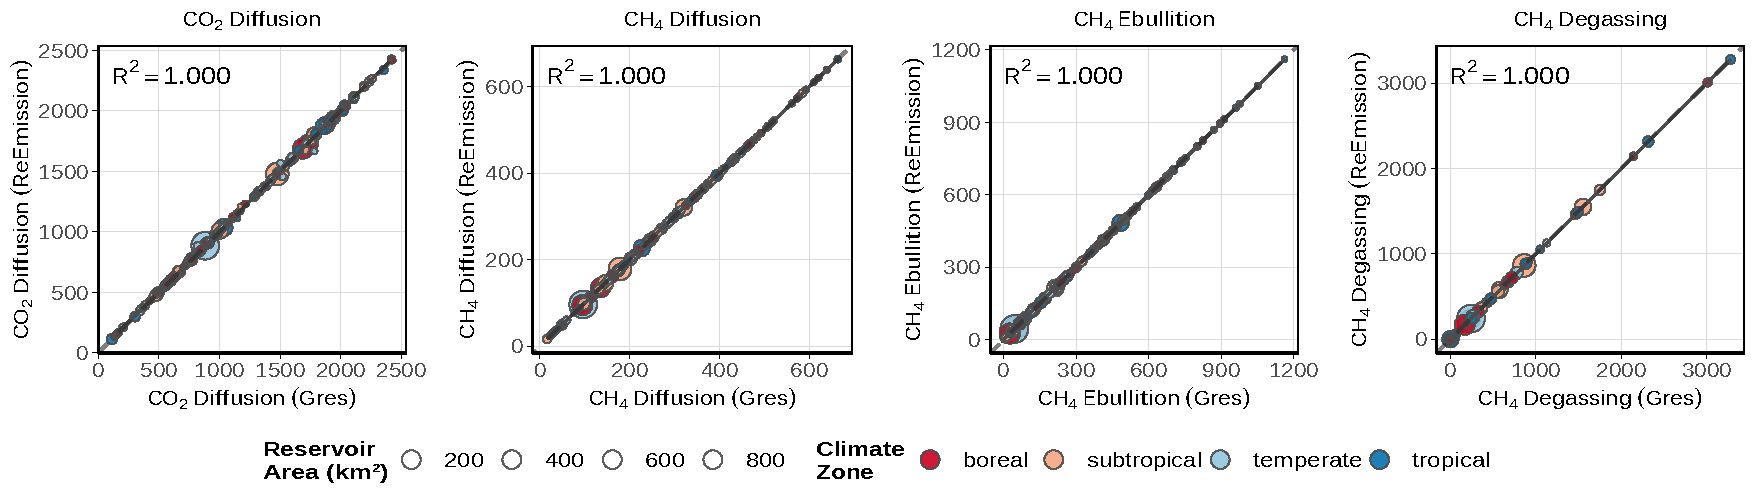
\includegraphics[width=1.0\textwidth]{figures/comparison_plot.pdf}
    \caption{{Comparison of gross areal emission fluxes (in gCO$_{2e}$ m$^{-2}$ yr$^{-1}$) via four emission pathways -- CO$_2$ diffusion, CH$_4$ diffusion, CH$_4$ ebullition, and CH$_4$ degassing (from left to right) -- predicted using Re-Emission (y-axis) and the R-based G-res implementation (x-axis).}}
    \label{fig:validation_plot_gross_emissions}
\end{figure}

\begin{figure}[ht]
    \centering
    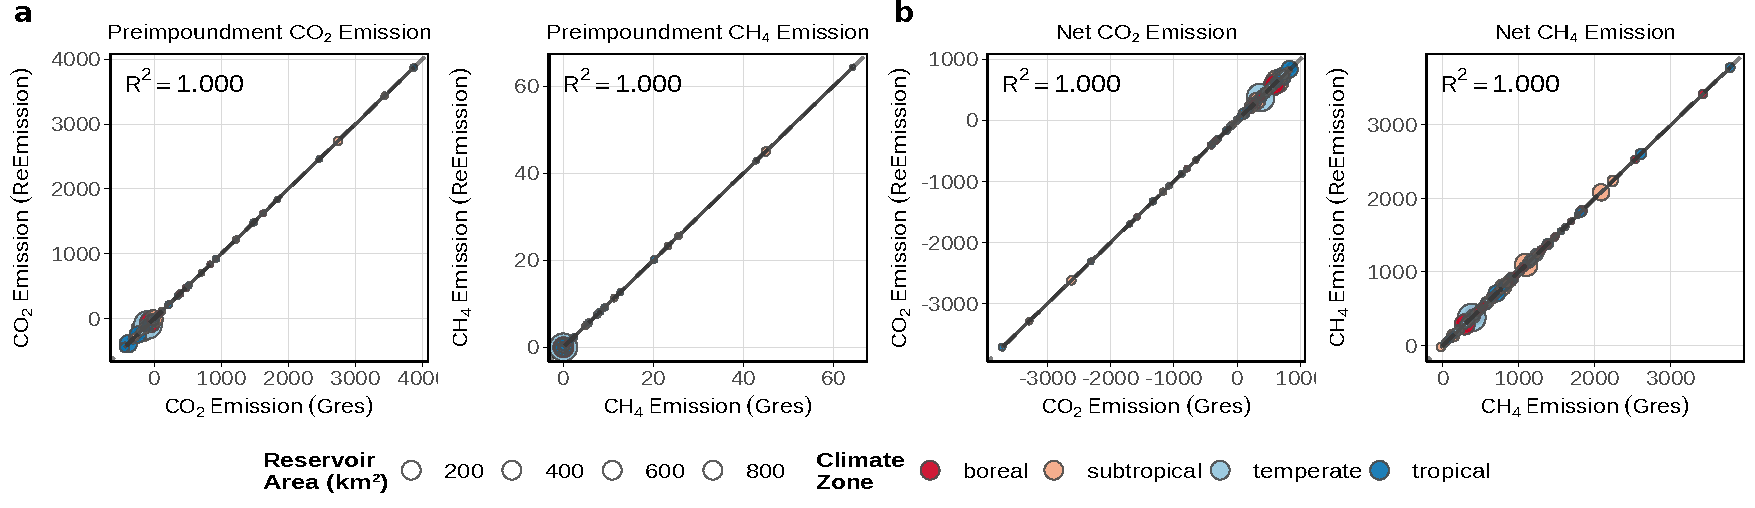
\includegraphics[width=1.0\textwidth]{figures/comparison_plot_net_emissions.pdf}
    \caption{{Comparison of (a) pre-impoundment CO$_2$ and CH$_4$ emissions (b) net anthropogenic CO$_2$ and CH$_4$ emissions per reservoir area (both in gCO$_{2e}$ m$^{-2}$ yr$^{-1}$) predicted using Re-Emission (y-axis) and the R-based G-res implementation (x-axis).}}
    
    \label{fig:validation_plot_net_emissions}
\end{figure}

\section{Case Studies}
\label{sec:case_studies}

Two case studies presented here demonstrate key functionalities of Re-Emission for predicting reservoir \ac{GHG} emissions: (i) estimation of emissions at scale, and (ii) quantification of emissions under parametric uncertainty.
The first case study illustrates how Re-Emission facilitates emission assessments across multiple reservoirs - e.g. regionally or nationally.
The second case study showcases the integration of Re-Emission with the Python-based sensitivity analysis library SALib~\cite{Iwanaga_Toward_SALib_2_0_2022}, enabling exploration of global sensitivity and uncertainty in emission predictions arising from uncertain model parameters.

This functionality has both practical and scientific value: it supports robust decision-making and contributes to methodological advancements in reservoir emission modelling.
To the best of our knowledge, the influence of uncertainties -- particularly input uncertainties -- on reservoir emission estimates has been examined only sparingly in the existing literature.
Re-Emission helps address this gap by enabling uncertainty and sensitivity analysis of emission models via SALib.
The source code for reproducing the results of both case studies is available on GitHub and archived on Zenodo -- see \emph{Data availability}.

\subsection{Emission trajectories from existing and planned assets in Myanmar}
\label{subsec:myanmar}

Using the Re-Emission framework, we estimated biogenic emissions from all identified \acf{IRR}, \acf{MP}, and \acf{HP} reservoirs in Myanmar known to us (approximately 200 in total).
For each reservoir, emission profiles -- representing the temporal evolution of biogenic emissions following impoundment -- were calculated and subsequently aggregated to derive national-scale reservoir emission trajectories.
This was achieved using Re-Emission's emission profile generation and aggregation module, which allows simulation and temporal aggregation of emissions from multiple reservoirs.
Emission trajectories were produced for multiple combinations of impoundment dates for existing and planned reservoirs lacking known commissioning dates, thereby quantifying the range of plausible national \ac{GHG} emission trajectories over a planning horizon.
Further methodological details are provided in the Materials and Methods section.

The ensemble results, illustrated in Figure~\ref{fig:mya_emission_profile}, reveal distinct temporal patterns across asset classes. 
Emissions from irrigation reservoirs appear to have peaked around 2005 and have declined steadily since, suggesting a maturing phase of irrigation infrastructure development. 
By contrast, emissions associated with planned \ac{HP} and \ac{MP} projects exhibit large uncertainty envelopes, reflecting substantial variation in potential commissioning timelines.
These projects are projected to drive a pronounced rise in national biogenic emissions, with peak values likely between 2030 and 2050. 
Although emissions are expected to decline sharply following this peak, they remain above present-day levels until at least 2060. 

Overall, the analysis indicates that future reservoir development has the potential to substantially alter Myanmar's national emission profile. 
This has direct policy relevance: Myanmar possesses over 100~GW of identified hydropower potential~\citep{EA_Myanmar} and aims to triple its hydropower capacity by 2030~\citep{Aung2020}, yet realizing this potential carries significant \ac{GHG} implications. 
The results presented in Figure~\ref{fig:mya_emission_profile} can support national mitigation planning and inform strategic infrastructure development.
Finally, Re-Emission's capability to dynamically alter model parameters enables straightforward extension of this analysis to other uncertainty types, such as parameter uncertainty, as demonstrated in the next case study.

\begin{figure}[ht]
    \centering
    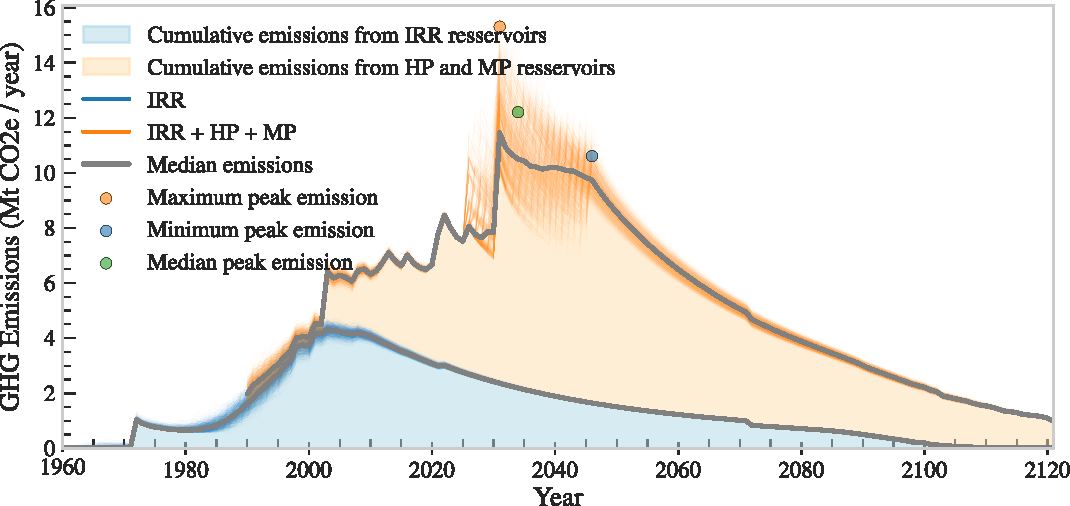
\includegraphics[width=0.8\textwidth]{figures/emission_profile.pdf}
    \caption{{Projected temporal evolution of emissions from existing and planned irrigation (IRR), multipurpose (MP), and hydroelectric (HP) reservoirs in Myanmar. In the absence of impoundment date information for some hydroelectric and multipurpose reservoirs, a 20-year planning horizon is assumed, by which all reservoirs included in current hydropower expansion plans are expected to be completed.}}
    \label{fig:mya_emission_profile}
\end{figure}

\subsection{Uncertainty analysis of reservoir emissions in Scotland and Wales}
\label{subsec:scotland_wales}

While it is widely recognised that reservoir emission models are subject to substantial uncertainty, the magnitude and origins of these uncertainties remain poorly characterised.
Emissions arise from complex biogeochemical processes that are difficult to observe and model due to their inherent spatio-temporal variability and and often poorly understood dynamics.
As a result, models built from limited observational data often exhibit notable epistemic and parametric uncertainties
Moreover, emission models depend on numerous input variables -- many derived from geospatial datasets -- which themselves carry variable degrees of uncertainty.
These factors lead to compounded uncertainty in model outputs, with direct implications for the reliability of emission estimates as a basis for decision-making and policy design.
Supporting systematic uncertainty analysis and probabilistic estimation under parameter and input uncertainty is therefore of clear practical value.

To demonstrate this functionality, we analysed parametric uncertainty in the G-res diffusive CO$_2$ and CH$_4$ emission models (Equations~\ref{eq:diff_co2_emission} and \ref{eq:diff_ch4_emission} respectively) and quantified its influence on total net anthropogenic emissions.
The analysis was intentionally limited to diffusive pathways, as the focus here is to illustrate the software's capability rather than to conduct a full quantitative sensitivity analysis.
The analysis was applied to 20 reservoirs located in Wales and Scotland. 

The results show that, of the two processes examined, uncertainty in total net emissions is dominated by CO$_2$ diffusion (Figure~\figref[b]{fig:uncertainty_analysis}), with highest sensitivity attributed to $k_{1 \; CO_2}^{diff}$ coefficient.
Coefficients $k_{6 \; CO_2}^{diff}$ and $k_{1 \; CH_4}^{diff}$ also contribute to output variability, although their influence differs across reservoirs.
This indicates that their importance is context-dependent, likely influenced by site-specific conditions or the relative contribution of individual emission pathways. 
Total net emissions and 95\% prediction intervals for all systems are shown in Figure~\figref[c]{fig:uncertainty_analysis}, again highlighting that prediction uncertainty is largely driven by CO$_2$ diffusion.
Figure~\figref[d]{fig:uncertainty_analysis} presents the probability density function of total net emissions for the Baddingsgill reservoir, illustrating the distribution of output values and indicating the mean, median, nominal estimate, and 5$^\textrm{th}$ and 95$^\textrm{th}$ percentiles.

Although this case study is intended primarily for demonstration, the workflow can be directly extended to incorporate a broader range of parametric and input uncertainties, both of which are supported.
%In practice, however, scaling Sobol-based analyses to larger sets of uncertain parameters may require access to high-performance computing resources due to their substantial computational cost.
Quantifying reservoir emissions under uncertainty remains an active area of research, and Re-Emission offers a flexible and extensible platform for developing and testing such analyses.

\begin{figure}[!h]
    \centering
    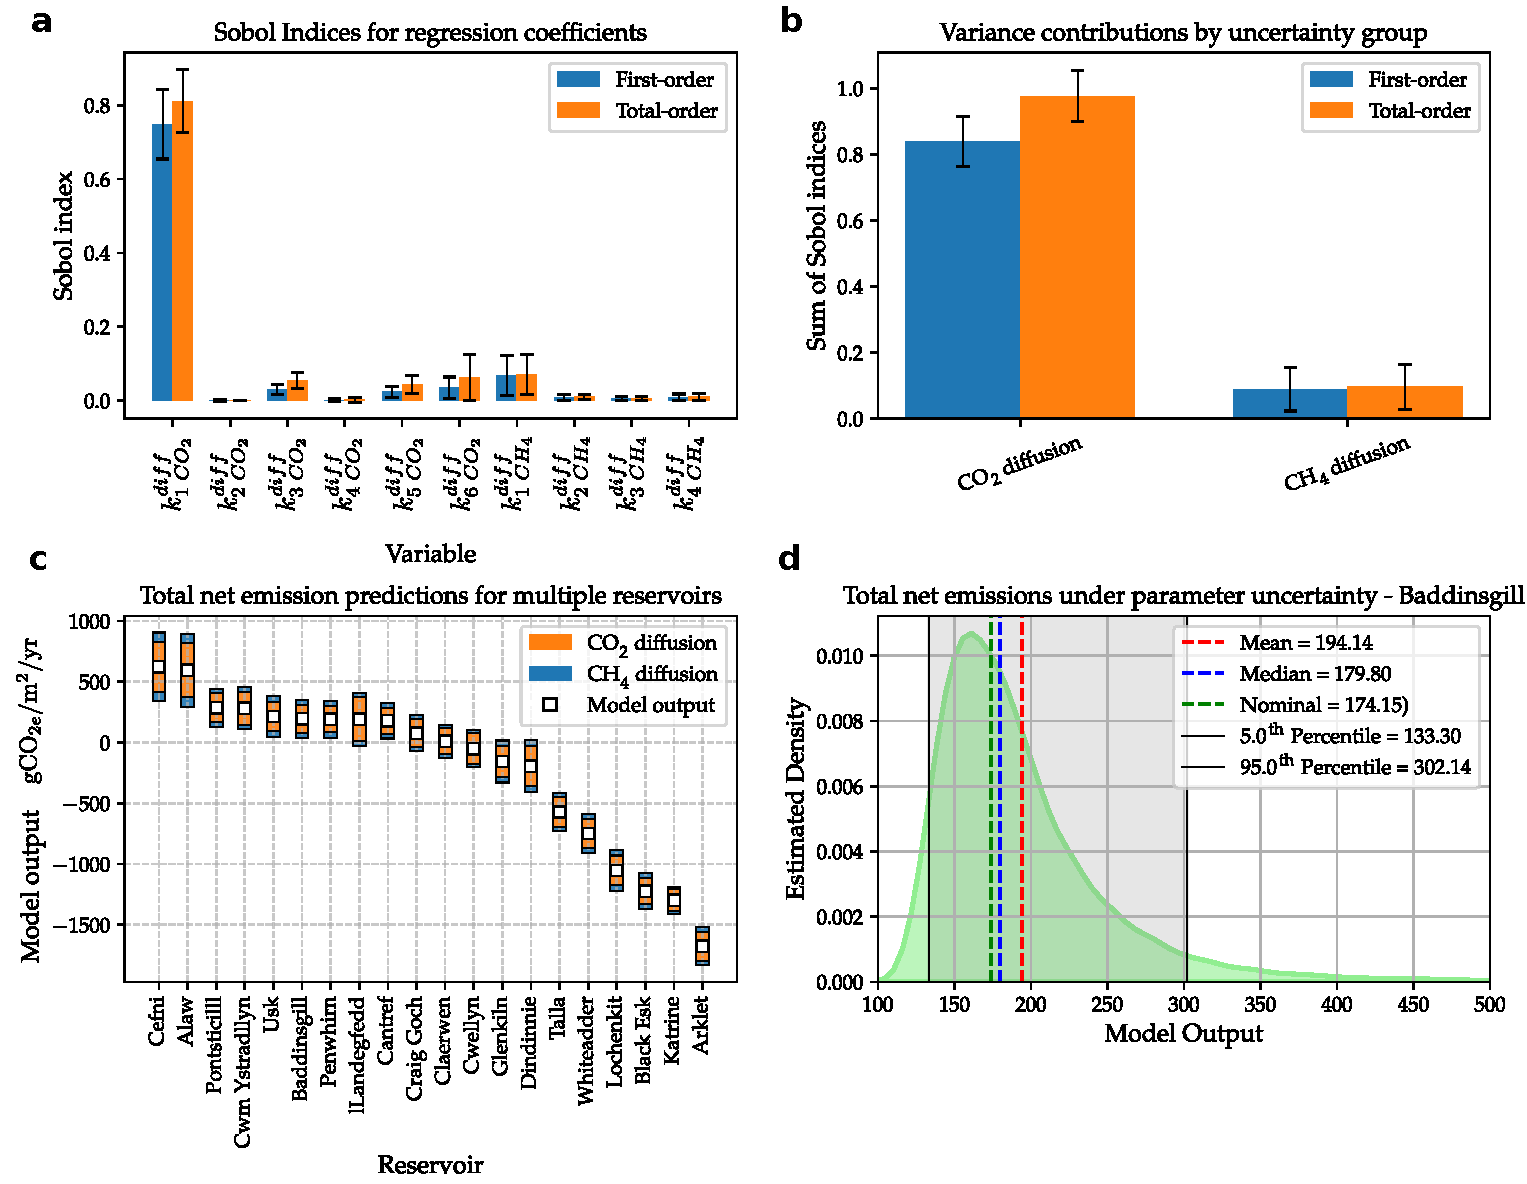
\includegraphics[width=1.0\textwidth]{figures/reemission_sobol_paper.pdf}
    \caption{
Quantification of parametric uncertainty in total net emissions from CO$_2$ and CH$_4$ diffusion processes for 20 reservoirs in Wales and Scotland. 
\textbf{(a)} First-order and total-order Sobol indices for the CO$_2$ and CH$_4$ diffusion regression coefficients, with error bars indicating variability across reservoirs. 
\textbf{(b)} Aggregated Sobol indices (first- and total-order) grouped by sources of uncertainty. 
\textbf{(c)} Total net emission estimates for the 20 reservoirs, with error bars indicating 95\% prediction intervals; the contribution of each uncertainty group is colour-coded. 
\textbf{(d)} Probability density function of total net emissions for a selected reservoir, with mean, median, nominal values, and the 5$^\textrm{th}$ and 95$^\textrm{th}$ percentiles indicated.
}
    \label{fig:uncertainty_analysis}
\end{figure}

\section{Discussion}
\label{sec:discussion}

This study addresses a key gap in existing tools, which has limited the ability to estimate reservoir \ac{GHG} emissions at scale, evaluate alternative model formulations, and integrate emission models into broader system-level analyses.
To overcome these limitations, we developed open-source software that implements and extends the G-res framework, enabling large-scale assessments of reservoir emissions through an interface with GeoCARET~\citep{heettool} -- an automated reservoir and catchment processing tool.
The software's capabilities were demonstrated in two case studies, illustrating its scalability, configurability, and support for advanced analyses such as uncertainty quantification and probabilistic modelling.
Although the tool represents a substantial step forward in modelling reservoir emissions, several limitations remain, motivating further development.
These limitations, along with benefits and directions for future work, are discussed below.

\subsection{Limitations}
\label{subsec:limitations}

Re-Emission is currently centred on implementing the G-res model and should not be interpreted as a general-purpose framework supporting a wide range of modelling paradigms (e.g., process-based or dynamic models).
Consequently, it inherits the biases, uncertainties, and limitations of G-res and relies primarily on static regression-based formulations.
For example, current G-res-based parameterizations exclude certain emission pathways observed in recent empirical research, including emissions linked to submerged macrophytes~\citep{Hilt2022, Suraj2023}.
Moreover, the underlying measurement data used for fitting the regression parameters are biased toward large, deep hydroelectric reservoirs~\citep{Hansen2022}, and therefore may not properly quantify emissions from smaller and shallower reservoirs which are often rich in organic matter, with greater littoral zone area fractions, and more conducive to elevated methane production~\citep{WANG2025123441, SHI2025}. 
% and downstream CH$_4$ degassing~\cite{Abbasi2020, Zhou2024}, which in some cases may account for a substantial share -- up to 90\% of total emissions~\cite{Deshmukh}. 

A second limitation relates to the current inability to simulate emissions from cascading reservoir systems, where the outflow of one reservoir forms the principal or partial inflow contribution to another. 
This limitation stems from both inherent constraints in the G-res model and the current architecture of the Re-Emission framework.
The implications can be potentially substantial for basin-scale and watershed-level analyses, particularly in regions where hydrologic connectivity and reservoir interactions shape carbon and nutrient transport, although, to our best knowledge, the magnitude of these effects remains unquantified.

Moreover, the N$_2$O model implementations are currently unvalidated and therefore experimental.
Users should consult the original publication by \citet{Maavara2019} for methodological caveats, noting in particular the model's sensitivity to the accuracy and stoichiometry of riverine nitrogen and phosphorus loads.
A variety of landscape nutrient export models are available, and many are region specific.
Therefore use of specific information, in particular land cover data, soil maps, land use / soil emission factors, is advocated where possible.

Finally, Re-Emission does not yet support emission models for other aquatic systems such as rivers and streams~\citep{Rocher-Ros2023}, lakes~\citep{Zhuang2023}, or wetlands~\citep{Hu2024}.
Although currently of minor practical significance, future applications will likely require multi-system integration and tools capable of integrated greenhouse gas and nutrient accounting across interconnected aquatic systems.

\subsection{Benefits}
\label{subsec:benefits}

Re-Emission advances reservoir \ac{GHG} modelling by providing a programmatic, scalable solution capable of batch processing and streamlined assessment across large reservoir inventories. 
It systematizes the workflow for the G-res framework and other prospective spatially explicit, and therefore conceptually similar models, defining a consistent structure for data handling, computation, and model evaluation.
Its modular open-source architecture allows users to extend the tool by adding new sub-models or applying custom parameterizations to existing model implementations -- an important direction highlighted by \citet{Pilla2025}.
Developed in Python, one of the most widely used languages in scientific and engineering programming, Re-Emission can be integrated into broader modelling pipelines.
This supports a wide set of applications, including the exploration of parametric and input uncertainty, and coupling with complementary tools such as GeoCARET for reservoir and catchment delineation, as demonstrated in this manuscript.
Finally, Re-Emission provides an open-source alternative to existing solutions, offering cost-free emission analysis for academic and most commercial users.
GeoCARET, however, may entail additional commercial-use costs owing to its reliance on Google Earth Engine (see Supplementary Materials).
Re-Emission's transparent, modular, and automated design promotes reproducibility, traceability, and ease of auditing in both research and applied settings.

\subsection{Future Work}
\label{subsec:future_work}

Future development of Re-Emission will address the limitations outlined in Section~\ref{subsec:limitations} by enhancing modularity, interoperability, and flexibility to facilitate implementation of new models and support next-generation reservoir \ac{GHG} assessments.

(i) Primary focus will be placed on decoupling the core framework from specific model implementations to establish Re-Emission as a fully generic emission-modelling platform.
We envisage an architecture in which composite models can be formulated by combining different submodels and data.
For example, phosphorus input to G-res could be defined either as a fixed quantity or derived dynamically from a phosphorus-export submodel.
This modular design would allow submodels to be introduced in place of fixed inputs, enabling complex coupled models to execute as a single-model.
The framework would simplify model construction through a high-level programming interface and support more controlled execution, for instance via one of the available open-source orchestration frameworks such as Dagster~\citep{dagster} or Prefect~\citep{prefect}.
This capability would also facilitate tighter, more formalized integration with upstream geospatial processing tools such as GeoCARET.

(ii) Transitioning to a more generic, modular framework will also enable introduction of process-based and dynamic models, e.g.~\cite{Soued2020exp, Delwiche2022}, moving beyond static regression approaches. 
This shift would help overcome some of the inherited G-res biases and support integration of currently excluded pathways such as macrophyte-mediated emissions and downstream degassing processes.
Integrating dynamic models may require additional model coupling interfaces that support dynamic execution, such as the Python framework for multi-agent simulation Pynsim~\citep{Knox2018_Pynsim}.

(iii) A key development priority for both this project and the broader research community is facilitating the representation of cascading reservoir systems. 
This capability could be enabled through a network-based architecture capable of representing interconnected reservoirs and river reaches.
Such a structure would permit explicit solution of carbon and nutrient mass balances and address current limitations in representing cascading systems, where nutrient and carbon transport are tightly coupled to hydrological connectivity yet these linkages remain unrepresented.
However, this transition will require development of new models most likely informed by additional empirical studies.
Consequently, developing globally applicable models for cascading reservoir systems with capabilities comparable to G-res will likely require sustained collaborative research effort.

(iv) An even longer-term objective involves extending the framework beyond reservoirs to toward integrated aquatic systems -- including rivers, wetlands, and lakes -- enabling comprehensive assessments of greenhouse gas and nutrient budgets across the land-to-ocean continuum (e.g.,\cite{Nixon2003,Maranger2018,Maavara2020}).
Coupling hydrodynamic models (e.g.,\cite{Almeida2022_temperatures,Long2019_Jinsha,He2025a}) with nutrient and carbon export models~\cite{He2025b} could enable representation of time-varying, non-steady-state conditions driven by climate change, land-use change, and reservoir operations (e.g.,\cite{Harrison2017}).
Deployment of such integrated frameworks will likely depend on availability of higher-resolution spatiotemporal data and improved process-level understanding (e.g.,\cite{grasset2021empirical}).

(v) Finally, future efforts will focus on modelling underrepresented emissions pathways and integrating additional \acp{GHG} -- notably nitrous oxide (N$_2$O), which remains the least characterized of the three dominant greenhouse gases emitted from aquatic systems.
Emerging evidence suggests that lakes and reservoirs may represent substantial global N$_2$O sources~\citep{Li2024}, and that under certain conditions N$_2$O emissions may rival or exceed those of CH$_4$~\citep{Chen2025}.
Other underrepresented pathways include emissions via submerged macrophytes~\citep{Hilt2022, Suraj2023}, downstream CH$_4$ degassing represented in more advanced models~\citep{Abbasi2020, Zhou2024}, and littoral zone emissions in response to wetting-drying cycles~\citep{Calamita2021, Ion2021}.
Incorporating these processes into modelling frameworks will be essential for accurately capturing the cumulative climate impacts of inland waters.

\section{Conclusions}
\label{sec:conclusions}

This work advances the standardization, transparency, and reproducibility of reservoir \acl{GHG} emission estimation.
By implementing the state-of-the-art G-Res model in an open-source Python environment, we offer a flexible platform for applying, extending, and testing emission models across diverse contexts.
Through integration with our reservoir and catchment analysis tool, we enable automated estimation of emissions across multiple reservoirs with minimal manual effort, as demonstrated in the two case studies.
Although some limitations remain and further development is required, the tool is already suited for practical applications, including assessments of individual reservoirs, regional and national inventories, and incorporation into broader modelling frameworks for strategic planning in the \ac{WEFE} nexus.
Our tool also aligns with the recommendations of the \emph{2019 Refinement to the 2006 \acs{IPCC} Guidelines for National Greenhouse Gas Inventories: Wetlands}~\citep{IPCC2019}, which encourage Tier~2 and Tier~3 approaches -- such as G-Res -- where sufficient data and analytical capacity exist.
By providing an open and extensible platform, this work supports ongoing efforts toward more consistent, transparent, and robust assessments of aquatic \ac{GHG} emissions.

\section{Software availability}
\label{sec:software_availability}
This paper describes the software in its current state of development, including all UML diagrams, code listings, and results.
All materials correspond to the \texttt{envsoft} branch of the Re-Emission GitHub repository and the \texttt{envsoft} branch of the Re-Emission-GeoCARET integration GitHub repository -- see detailed information about both packages below.
The Re-Emission GitHub repository includes a collection of interactive Jupyter Notebooks that demonstrate the use of the software and complement the code listings presented in this manuscript.
These notebooks are available in the \texttt{examples} directory of the GitHub repository.

\begin{description}
  \item[\textbf{Name of the software:}] \texttt{Re-Emission}
  \item[\textbf{Developers:}] Tomasz Janus
  \item[\textbf{Contact address:}] \href{mailto:tomasz.janus@manchester.ac.uk}{tomasz.janus@manchester.ac.uk}, \href{mailto:tomasz.k.janus@gmail.com}{tomasz.k.janus@gmail.com}
  \item[\textbf{Year first available:}] 2022
  \item[\textbf{Hardware required:}] Windows 7, 10 (tested), 11, Linux (tested on Ubuntu 22.04), MacOSX
  \item[\textbf{Software required:}] \LaTeX \, (optional)
  \item[\textbf{Program language:}] Python 3.10+
  \item[\textbf{License:}] GNU General Public Licence v3
  \item[\textbf{Availability and cost:}] free and open source
  \item[\textbf{Source code:}] \href{https://github.com/tomjanus/reemission/tree/envsoft}{https://github.com/tomjanus/reemission/tree/envsoft} %and \href{https://pypi.org/project/pyclmuapp}{PyPI}
  %\item[\textbf{Distribution:}] \hl{Put on PyPi and maybe also on conda-forge if straightforward to do - in case we do both, add two entries: Distribution (PyPi) and Distribution (conda-forge)}
  \item[\textbf{Documentation:}] \href{https://tomjanus.github.io/reemission}{https://tomjanus.github.io/reemission}
\end{description}

\vspace{3pt}

\begin{description}
  \item[\textbf{Name of the software:}] \texttt{Re-Emission GeoCARET Integration}
  \item[\textbf{Developers:}] Tomasz Janus
  \item[\textbf{Contact address:}] \href{mailto:tomasz.janus@manchester.ac.uk}{tomasz.janus@manchester.ac.uk}, \href{mailto:tomasz.k.janus@gmail.com}{tomasz.k.janus@gmail.com}
  \item[\textbf{Year first available:}] 2024
  \item[\textbf{Hardware required:}] Platform-independent
  \item[\textbf{Software required:}] Docker, \LaTeX \, (optional)
  \item[\textbf{Program language:}] YAML configuration
  \item[\textbf{License:}] GNU General Public Licence v3
  \item[\textbf{Availability and cost:}] free and open source, requires Google Earth Engine and Google Cloud registrations which might incur costs for commercial use cases
  \item[\textbf{Source code:}] \href{https://github.com/tomjanus/geocaret-reemission/tree/envsoft}{https://github.com/tomjanus/geocaret-reemission/tree/envsoft}
\end{description}

\section{Data availability}
\label{sec:data_availability}

The Re-Emission code is open-source and freely available on GitHub (see \emph{Software Availability}).
The manuscript source files in \LaTeX, including all figures, as well as the Jupyter Notebooks in Python and R used to run the case studies and produce results case study and Re-Emission model validation plots, are provided at: \href{https://github.com/tomjanus/reemission-paper}{https://github.com/tomjanus/reemission-paper}.
The above repository contains all data and scripts necessary to reproduce the results presented in this manuscript. 
Additionally, the complete repository -- including intermediate and final outputs -- has been archived on Zenodo: \href{https://doi.org/10.5281/zenodo.16424011}{doi:10.5281/zenodo.16424011}.

\section{CRediT authorship contribution statement}
\textbf{Tomasz Janus:} Conceptualization, Methodology, Formal analysis, Investigation, Visualization, Software -- Re-Emission, Re-Emission GeoCARET integration, and Case Studies, Data Curation, Writing -- original draft, Writing -- review \& editing.
\textbf{Christopher Barry:} Conceptualization, Methodology, Software -- Model Validation, Writing -- review \& editing, Investigation -- Model Validation against G-res Tool v3.31.
\textbf{Xingxing Zhang:} Software Validation and Testing, Writing -- review \& editing.
\textbf{Jaise Kuriakose:} Conceptualization, Methodology, Writing -- review \& editing, Funding acquisition, Project Administration.

\section{Declaration of competing interest}
The authors declare that they have no known competing financial interests or personal relationships that could have appeared to influence the work reported in this paper.

\section{Acknowledgements}
The authors would like to acknowledge the assistance provided by the Research IT Group at the University of Manchester, in particular James Sinnott, for their help in containerizing our software using Docker.
The development of the methodology and of the early version of Re-Emission and the Myanmar case study was supported by the UK Economic and Social Research Council's Global Challenges Research Fund (GCRF) as part of the UK Research and Innovation (UKRI) Funded FutureDAMS project(\href{www.futuredams.org}{ES/P011373/1}).
Work on containerising Re-Emission and Re-Emission GeoCARET integration was partially funded by UoM's Open Research Accelerator fund.
The case study on emission uncertainty quantification for UK reservoirs was funded by UoM's Policy@Manchester fund.
Further funding for T.J., J.K.and X.Z. was provided by their institutions. 
The work of C.B. was supported by the UK Centre for Ecology and Hydrology (UKCEH). 
Any opinions, findings, and conclusions or recommendations expressed in this material are those of the authors but not necessarily the funders.

%% The Appendices part is started with the command \appendix;
%% appendix sections are then done as normal sections
\appendix

\section{Selected Code Listings}
\label{app1}

\begin{minipage}{\textwidth}
\begin{lstlisting}[language=PythonReemission, label={lst:em_calc_setup}, caption={Use of Re-Emission as a library: step-by-step problem formulation.}]
from reemission.temperature import MonthlyTemperature
from reemission.emissions   import CarbonDioxideEmission, NitrousOxideEmission, MethaneEmission
from reemission.constants   import Landuse, Climate, SoilType, Biome, TreatmentFactor, LanduseIntensity
from reemission.catchment   import Catchment
from reemission.reservoir   import Reservoir
from reemission.biogenic    import BiogenicFactors

mt = MonthlyTemperature(
  [10.56,11.99,15.46,18.29,20.79,22.09,
   22.46,22.66,21.93,19.33,15.03,11.66])
coordinates = [22.6, 94.7] # Latitude and Longitude
biogenic_factors    = BiogenicFactors(
  biome             = Biome.TROPICALMOISTBROADLEAF,
  climate           = Climate.TROPICAL,
  soil_type         = SoilType.MINERAL,
  treatment_factor  = TreatmentFactor.NONE,
  landuse_intensity = LanduseIntensity.LOW)
catchment_area_fractions = \
  [0.0, 0.0, 0.0, 0.0, 0.0, 0.01092, 0.11996, 0.867257, 0.0]
reservoir_area_fractions = [
  0.0, 0.0, 0.0, 0.0, 0.0, 0.45, 0.15, 0.4, 0.0, 
  0.0, 0.0, 0.0, 0.0, 0.0, 0.0,  0.0,  0.0, 0.0, 
  0.0, 0.0, 0.0, 0.0, 0.0, 0.0,  0.0,  0.0, 0.0]
catchment_inputs = {
  'runoff'     : 1685.6, 'area'         : 78203, 'population' : 8463, 
  'riv_length' : 9.2,    'slope'        : 8.0,   'precip'     : 2000,   
  'etransp'    : 400,    'soil_wetness' : 140,   'mean_olsen' : 5.85, 
  'biogenic_factors' : biogenic_factors,
  'area_fractions'   : catchment_area_fractions}
reservoir_inputs = {
  'volume'       : 7.66E6, 'area': 100.6,       'max_depth'         : 32.0, 
  'mean_depth'   : 13.6,   'soil_carbon': 10.2, 'water_intake_depth': 20.0
  'mean_radiance': 4.5,    
  'mean_monthly_windspeed': 3.8, 'mean_radiance_may_sept': 4.5, 
  'mean_radiance_nov_mar' : 3.2, 'area_fractions': reservoir_area_fractions
}    
year_profile = (1, 5, 10, 20, 30, 40, 50, 65, 80, 100)
catchment = Catchment(**catchment_inputs)
reservoir = Reservoir(
  **reservoir_inputs,        temperature = mt,
  coordinates = coordinates, inflow_rate = catchment_1.discharge)
\end{lstlisting}
\end{minipage}

\begin{minipage}{\linewidth}
\begin{lstlisting}[language=PythonReemission, label={lst:em_calc}, caption={Use of Re-Emission as a library: calculation of CO$_2$ and CH$_4$ emissions using \texttt{CarbonDioxideEmission} and \texttt{MethaneEmission} classes.}]
em_co2 = CarbonDioxideEmission(
  catchment = catchment_1,            reservoir     = reservoir_1,
  eff_temp  = mt.eff_temp(gas='co2'), p_calc_method = 'g-res')
co2_emission_profile = em_co2.profile(years = year_profile)
co2_emission_factor  = em_co2.factor()    # Gross emission flux
co2_net_total        = em_co2.net_total() # Net anthropogenic emission flux
em_ch4 = MethaneEmission(
	catchment = catchment_1, reservoir = reservoir_1, monthly_temp = mt)
ch4_ebullition       = em_ch4.ebullition_flux_int() # Gross ebullition flux
ch4_emission_factor  = em_ch4.diffusion_flux_int()  # Gross diffusion flux
ch4_degassing_flux   = em_ch4.degassing_flux_int()  # Gross degassing flux
\end{lstlisting}
\end{minipage}

\begin{minipage}{\linewidth}
\begin{lstlisting}[language=PythonReemission, label={lst:em_calc_file}, caption={Use of Re-Emission as a library: calculation of reservoir emissions with inputs read from file using the \texttt{Input} class.}]
from reemission.input import Inputs
from reemission.model import EmissionModel
from reemission.utils import get_package_file
input_data    = Inputs.fromfile('inputs.json')
output_config = get_package_file('config', 'outputs.yaml').as_posix()
model         = EmissionModel(
  inputs  = input_data, 
  config  = output_config, 
  p_model = 'g-res'
)
model.calculate()
print(model.outputs)
\end{lstlisting}
\end{minipage}

\begin{minipage}{\linewidth}
\begin{lstlisting}[language=PythonReemission, label={lst:em_calc_presentation}, caption={Use of Re-Emission as a library: saving results in multiple file formats using the \texttt{Presenter} and \texttt{Writer} classes.}]
from reemission.presenter import JSONWriter, LatexWriter, HTMLWriter
model.add_presenter(
  writers=[JSONWriter, LatexWriter, HTMLWriter, ExcelWriter],
  output_files=['output.json', 'output.pdf', 'output.html', 'output.xlsx'])
model.calculate()
model.save_results()
\end{lstlisting}
\end{minipage}

\begin{figure}[ht]
    \centering
    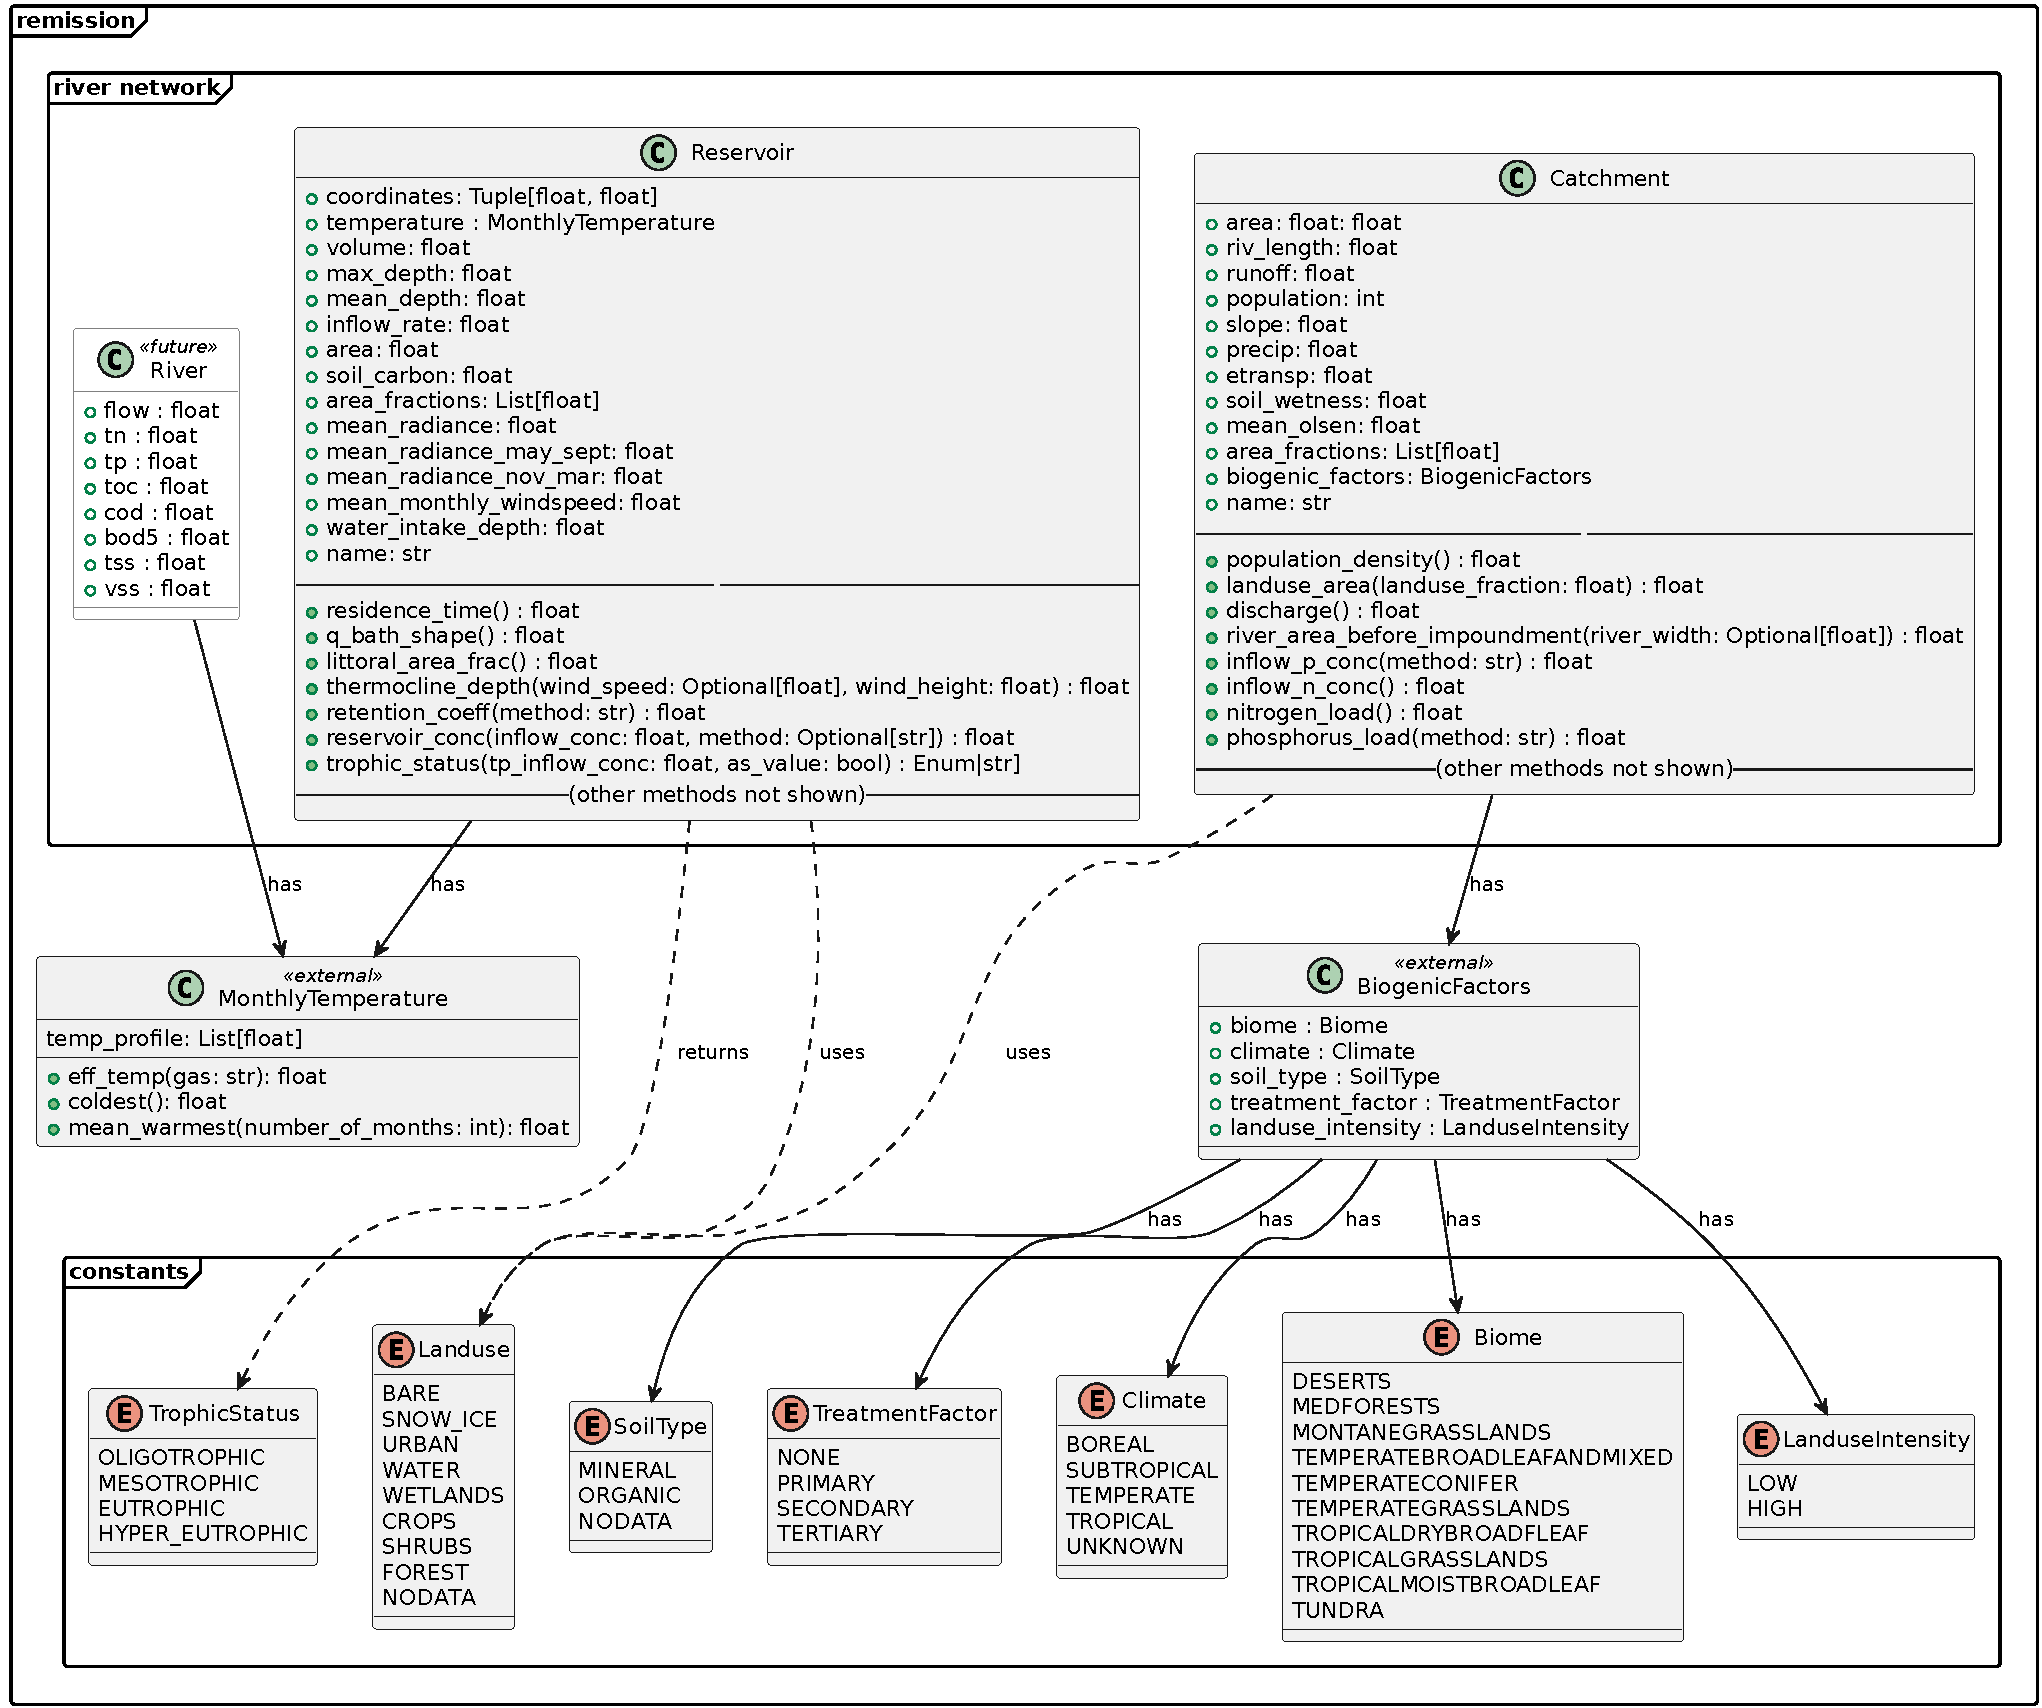
\includegraphics[width=0.99\textwidth]{figures/river_network_uml.pdf}
    \caption{A UML class diagram visualizing the \vrbbrk{Reservoir} and \vrbbrk{Catchment} classes and different container classes and categorical data representations using Enum classes.}
    \label{fig:river_network_emissions_uml}
\end{figure}

\begin{figure}[ht]
    \centering
    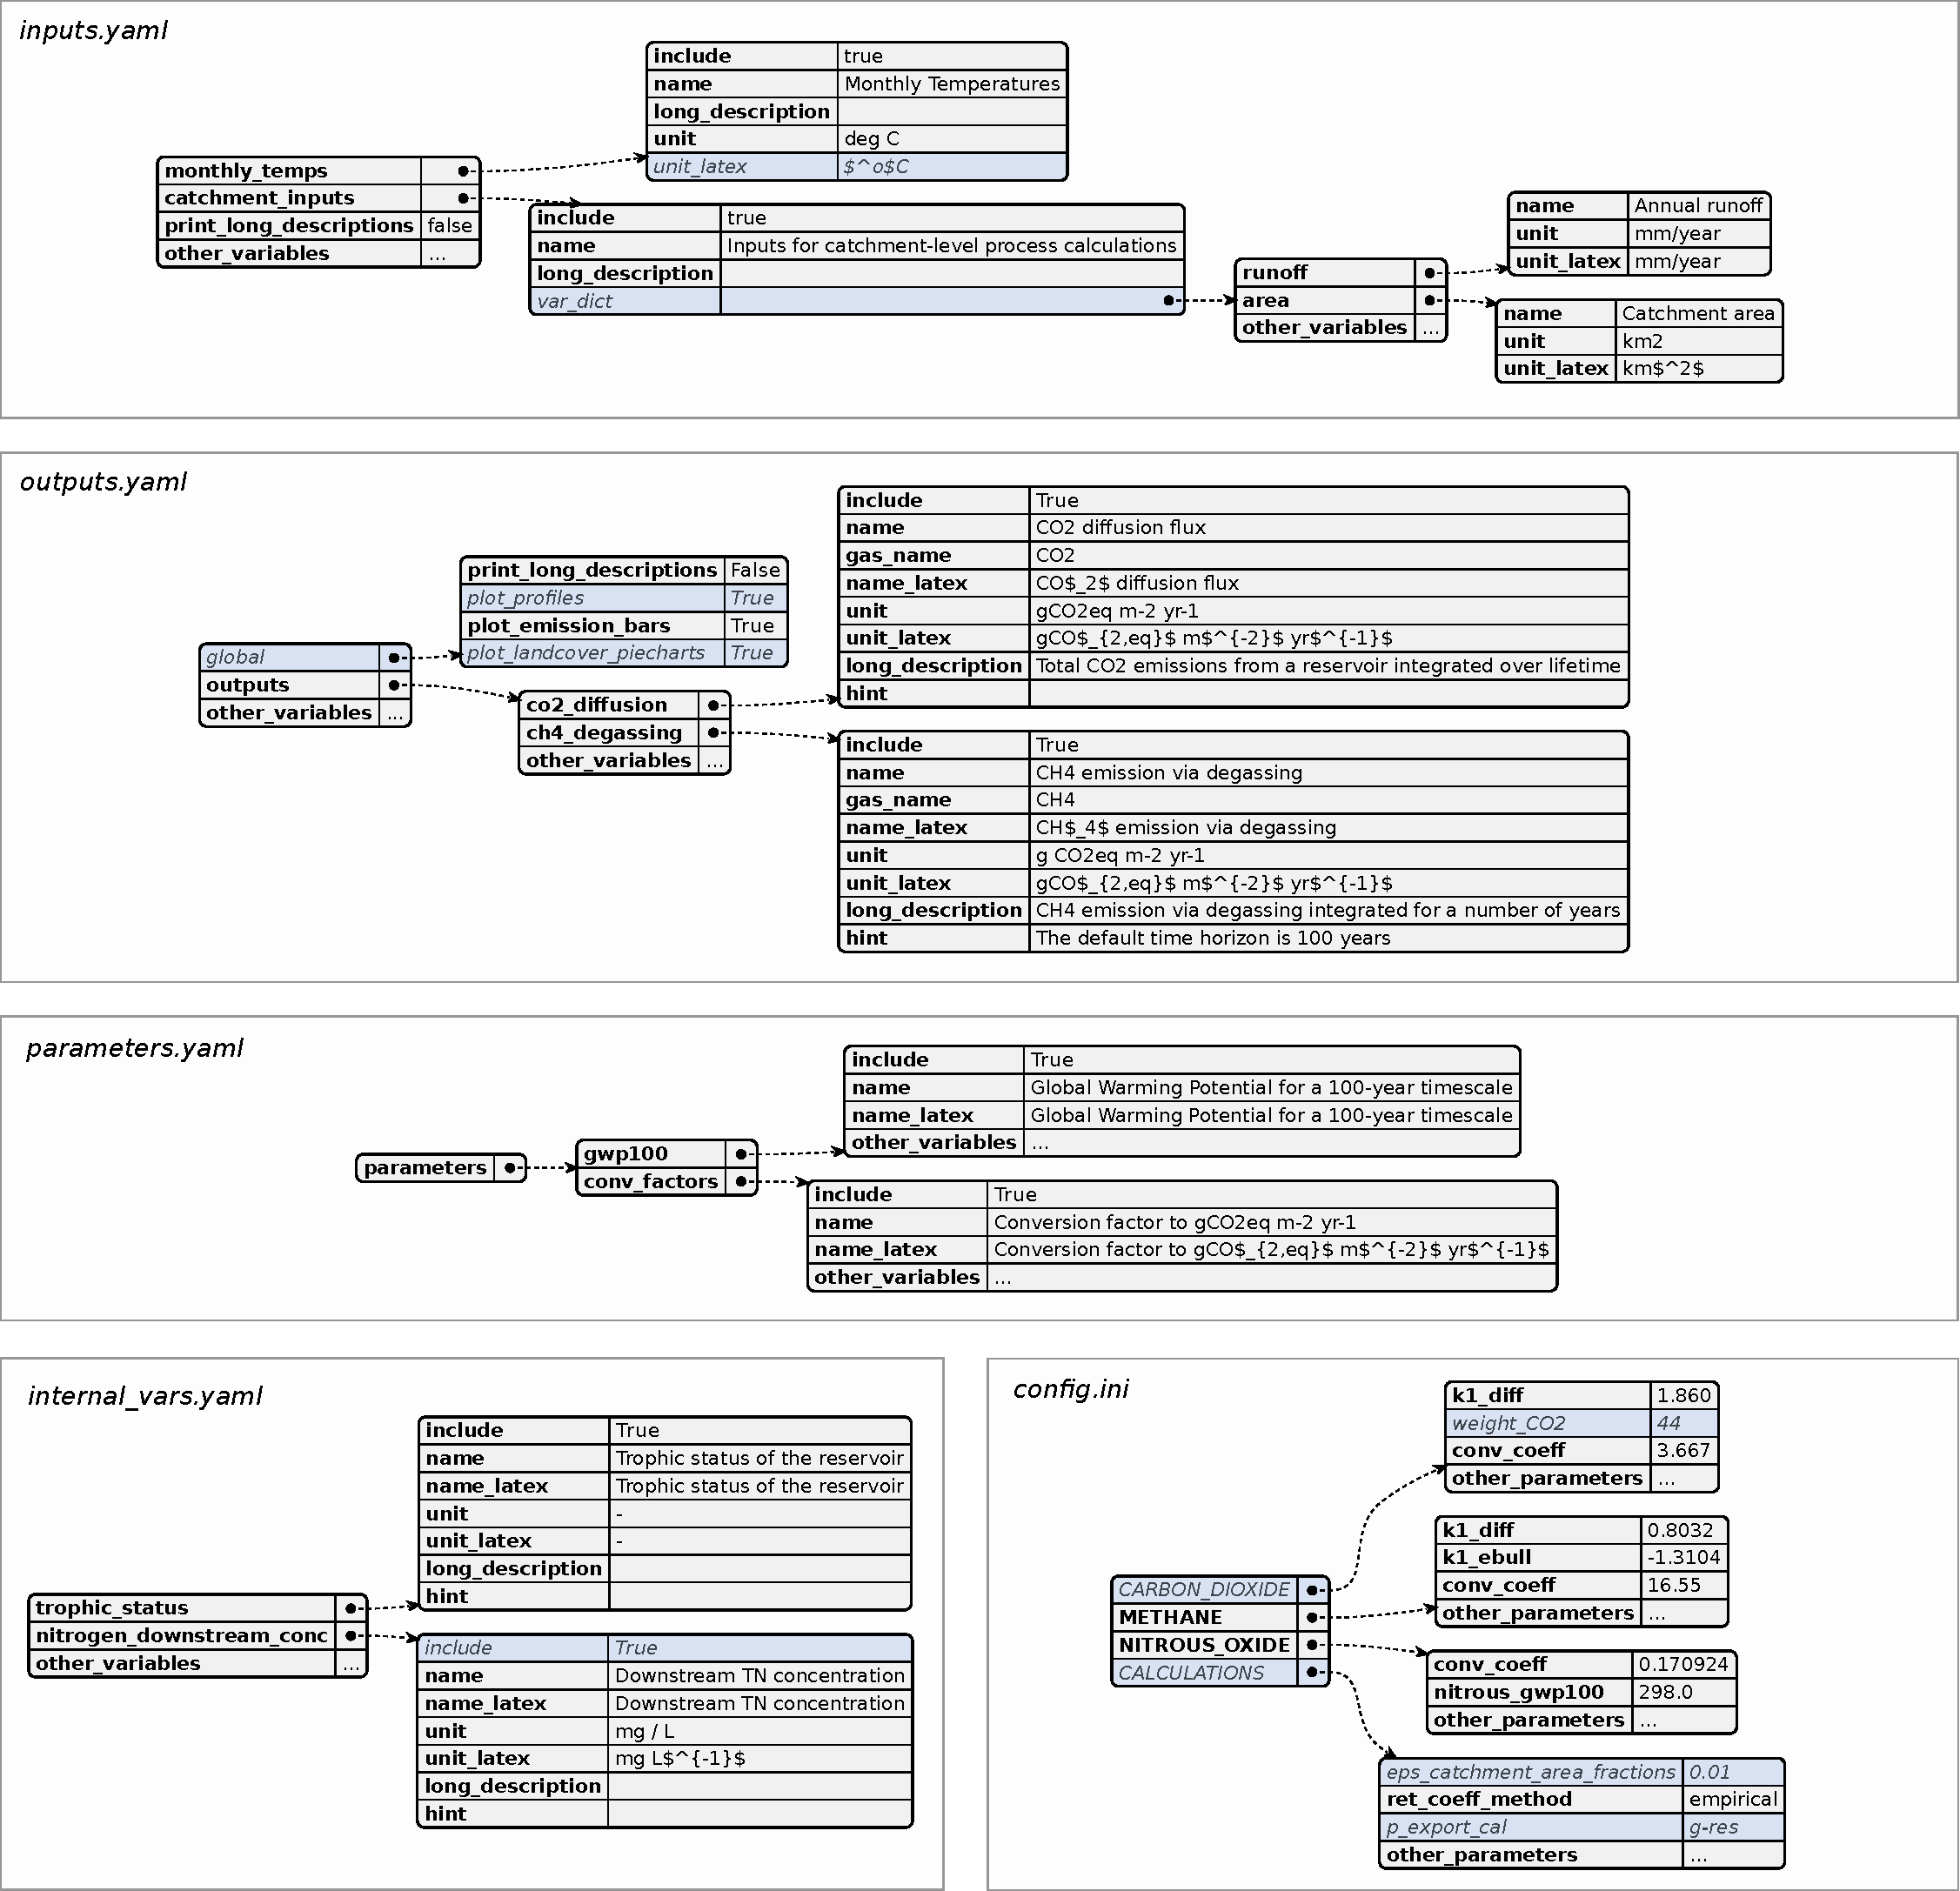
\includegraphics[width=0.99\textwidth]{figures/config_uml_portrait.pdf}
    \caption{Diagrams illustrating the structure of YAML configuration files used by the Presenter class (\vrbbrk{inputs.yaml}, \vrbbrk{outputs.yaml}, \vrbbrk{parameters.yaml}, \vrbbrk{internal\_vars.yaml}), along with the \vrbbrk{config.ini} file specifying emission model parameters and selection of alternative models.}
    \label{fig:config_uml}
\end{figure}

\begin{figure}[ht]
    \centering
    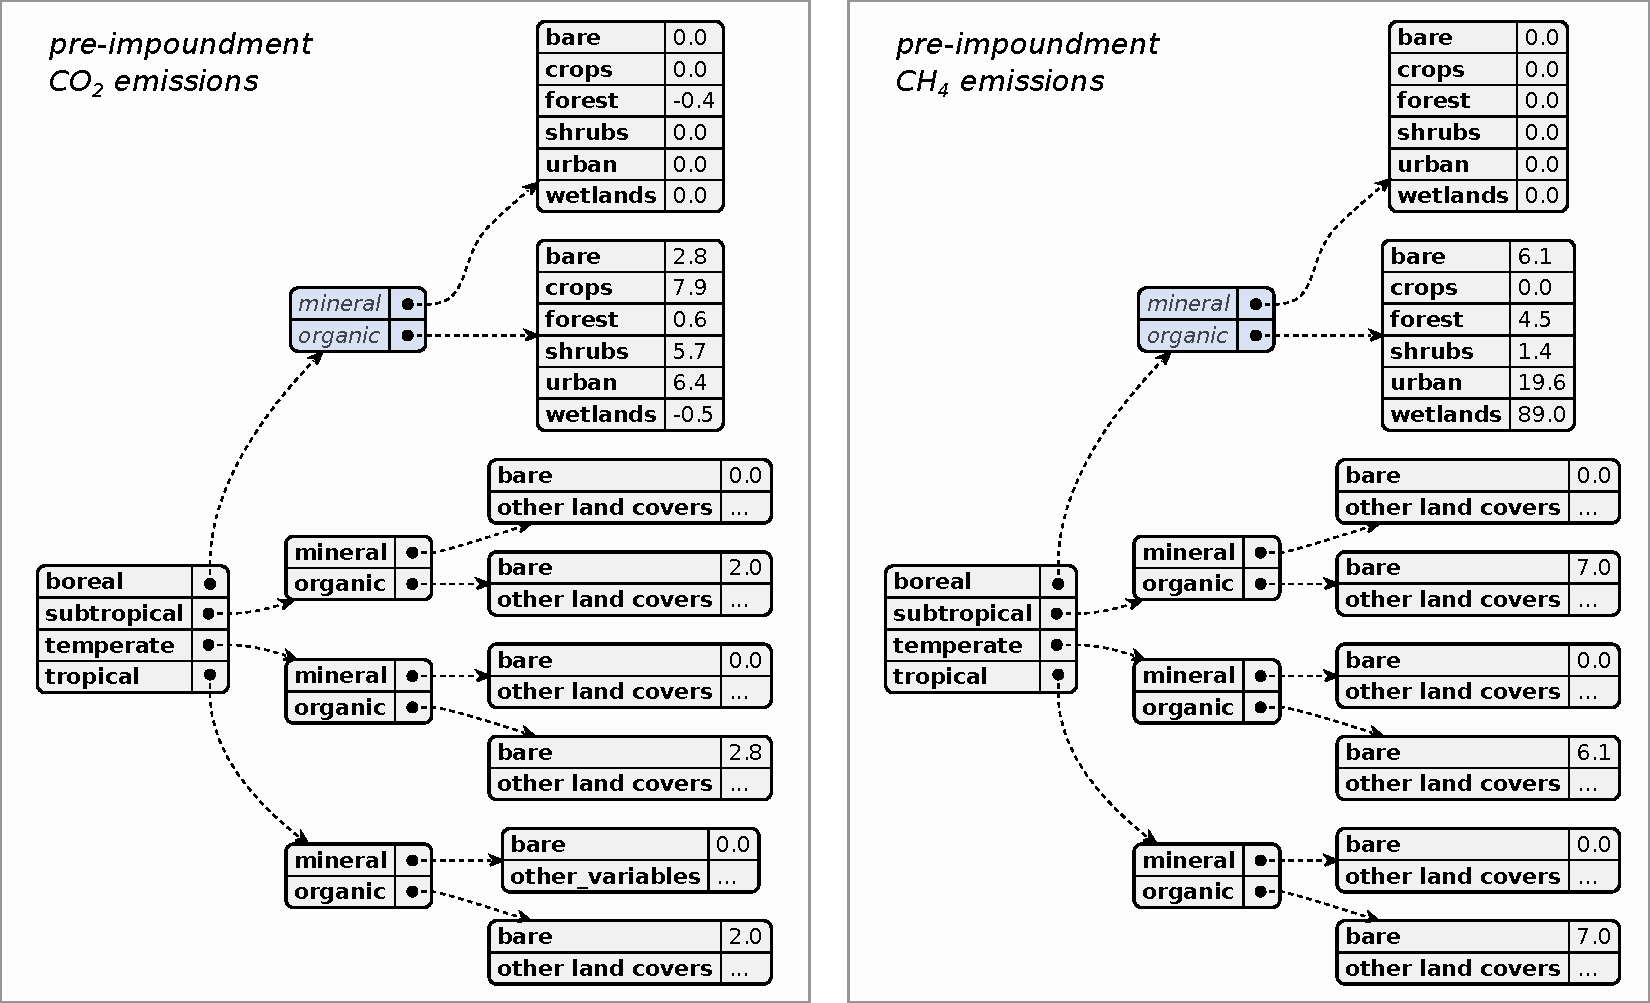
\includegraphics[width=0.80\textwidth]{figures/preimpoundment.pdf}
    \caption{Diagrams illustrating the structure of YAML configuration files and the underlying data relating areal pre-impoundment CO$_2$ and CH$_4$ emissions to climate, soil type, and land cover type.}
    \label{fig:preimpoundment}
\end{figure}

\begin{figure}[ht]
    \centering
    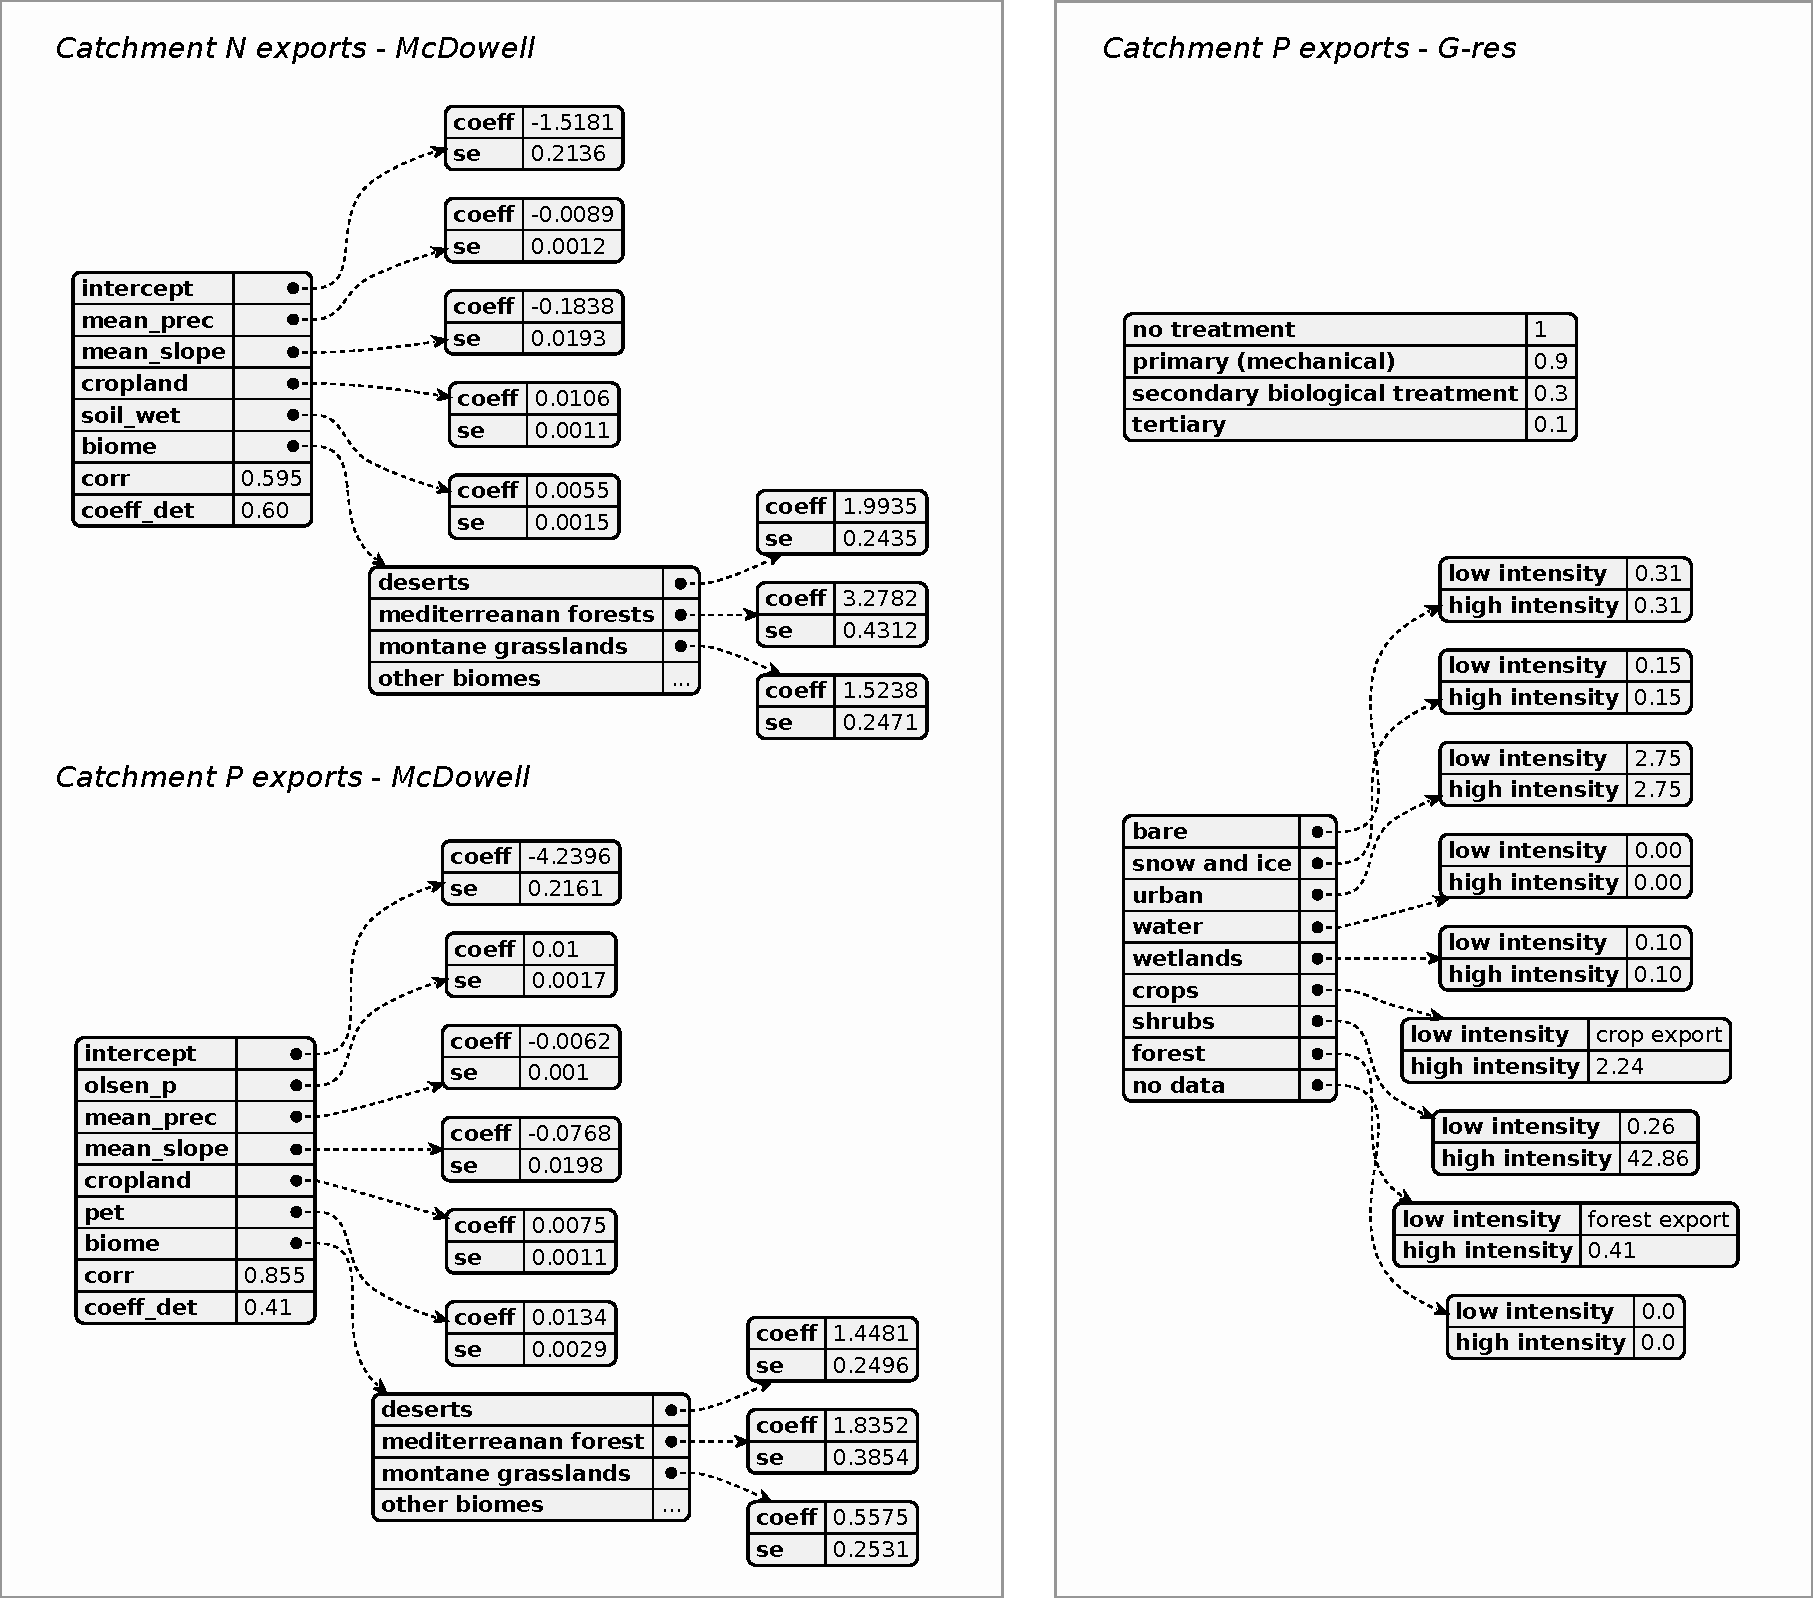
\includegraphics[width=0.85\textwidth]{figures/tp_tn_exports.pdf}
    \caption{Diagrams illustrating the structure of YAML configuration files parameterizing the nutrient export models of \citet{McDowell2020} (\ac{N} and \ac{P}) and G-res (\ac{P}).}
    \label{fig:tp_tn_exports}
\end{figure}

\begin{table}[ht]
\begin{threeparttable}
    \label{app_table:input_variables}
	{\small
    \caption{Input variables used by Re-Emission for estimating \ac{GHG} emissions from reservoirs. Additional details on the geospatial data sources used to derive these inputs are provided in Supplementary Tables 4 and 5 in \citet{janus2025planning}.}
    \label{app_table:input_variables}%
    \begin{tabular*}{\linewidth}{@{\extracolsep{\fill}}lcc@{}}
    \toprule
    Input Name & Unit & Model\tnote{2} \\
    \midrule%
    \multicolumn{3}{c}{Inputs for catchment{-}level calculations}\\%
    %\midrule%
    Biome&{-} & McDowell\tnote{3}\\%
    Climate&{-} & G-res\\%
    Soil Type&{-} & -\tnote{4}\\%
    Treatment Factor&{-} & G-res\\%
    Landuse Intensity&{-} & G-res\\%
    Monthly Temperatures&$^o$C & G-res\\%
    Annual runoff&mm/year & G-res\\%
    Catchment area&km$^2$ & G-res\\%
    Length of inundated river&km & G-res\\%
    Population&capita & G-res\\%
    Area fractions\tnote{1}&--& G-res, McDowell\tnote{3}\\%
    Mean catchment slope&\%& McDowell\tnote{3}\\%
    Mean annual precipitation&mm/year& McDowell\tnote{3}\\%
    Mean annual evapotranspiration&mm/year& McDowell\tnote{3}\\%
    Soil wetness&mm over profile& McDowell\tnote{3}\\%
    Soil Olsen P content&kgP ha$^{-1}$& McDowell\tnote{3}\\%
    \midrule%
    \multicolumn{3}{c}{Inputs for reservoir{-}level calculations}\\%
    %\midrule%
    Reservoir volume&m$^3$& G-res\\%
    Reservoir area&km$^2$& G-res\\%
    Maximum reservoir depth&m& G-res\\%
    Mean reservoir depth&m& G-res\\%
    Inundated area fractions\tnote{1}&-& G-res\\%
    Soil carbon in inundated area&kgC m$^{-2}$& G-res\\%
    Mean monthly horizontal radiance&kWh m$^{-2}$ d$^{-1}$& G-res\\%
    Mean monthly horizontal radiance: May {-} Sept&kWh m$^{-2}$ d$^{-1}$& G-res\\%
    Mean monthly horizontal radiance: Nov {-} Mar&kWh m$^{-2}$ d$^{-1}$& G-res\\%
    Mean monthly wind speed&m s$^{-1}$& G-res\\%
    Water intake depth below surface&m& G-res\\
    \bottomrule
    \end{tabular*}
    }
    {\noindent
    \begin{tablenotes}
        \footnotesize
        \item{1} Fractions of land cover in the delineated area.
        \item{2} Model implementations relying on the input variable.
        \item{3} Land nitrogen (N) and phosphorus (P) export model by McDowell et al.~\cite{McDowell2020}. P exports can serve as an alternative estimate of total P load for the G-res model, while nitrogen exports are used to inform nitrous oxide (N$_2$O) emission models.
        \item{4} Included for informational purposes only and not used as a predictive input in any of the implemented models.
    \end{tablenotes}
    }
\end{threeparttable}
\end{table}

%\FloatBarrier

\begin{acronym}
	\acro{ASEAN}{Association of Southeast Asian Nations}
	\acro{BRT}{Boosted Regression Tree}
	\acro{CO2}[CO$_2$]{carbon dioxide}
	\acro{CH4}[CH$_4$]{methane}
	\acro{CI}{continuous integration}
	%\acro{CI}{carbon intensity}
	\acro{CLI}{command line interface}
	\acro{DEM}{digital elevation model}
	\acro{DFS}{depth-first search}
	\acro{DOC}{dissolved organic carbon}
	\acro{DOF}{degree of fragmentation}
	\acro{DOR}{degree of regulation}
	\acro{EF}{emission factor}
	\acro{EFDC}{Environmental Fluid Dynamics Code}
	\acro{EI}{emission intensity}
	\acro{EPA}{U.S. Environmental Protection Agency}
	\acro{ET}{evapotranspiration}
	\acro{FHReD}{High-Resolution Global Database of Dams}
	\acro{FSL}{full supply level}
	\acro{GDrive}{Google Drive}
	\acro{GGRP}{Greenhouse Gas Reporting Program}
	\acro{GEE}{Google Earth Engine}
	\acro{GHCR}{GitHub Container Registry}
    \acro{GHG}{greenhouse gas}    
	\acro{GIS}{geographical information system}
	\acro{G-res}{GHG Reservoir Tool}
	\acro{GOOD2}{Global geOreferenced Database of Dams}
	\acro{GW}{gigawatts}
	\acro{HP}{hydropower}
	\acro{ICOLD}{International Commission on Large Dams}
	\acro{IHA}{International Hydropower Association}
	\acro{IRR}{irrigation}
	\acro{KDE}{kernel density estimate}
	\acro{IPCC}{Intergovernmental Panel on Climate Change}
	\acro{KNN}{K-Nearest Neighbours Regressor}
	\acro{LCA}{life-cycle assessment}
	\acro{ML}{machine-learning}
	\acro{MP}{multipurpose}
	\acro{MW}{megawatts}
	\acro{MOEA}{multiobjective evolutionary algorithm}
	\acro{MOO}{multiobjective optimization}
	\acro{N}{Nitrogen}
	\acro{N2O}[N$_2$O]{nitrous oxide}
	\acro{P}{Phosphorus}
	\acro{PD}{partial-dependence}
	\acro{PPA}{power purchase agreement}
	\acro{PV}{Photovoltaic}
	\acro{RF}{Random Forest}
	\acro{ROI}{region of interest}
	\acro{RoR}{run-of-river}
	\acro{RMSE}{root-mean-square-error}
	\acro{SA}{sensitivity analysis}
	\acro{SDG}{sustainable development goal}
	\acro{SES}{social and ecological system}
	\acro{SVR}{Support Vector Regression}
	\acro{xAI}{explainable artificial-intelligence}
	\acro{TN}{Total Nitrogen}
	\acro{TP}{Total Phosphorus}
	\acro{UAS}{Unrelated Anthropogenic Sources}
    \acro{VRE}{variable renewable energy}
	\acro{WEFE}{Water-Energy-Food-Ecosystems}
	\acro{WRT}{water residence time}
\end{acronym}

\bibliographystyle{unsrtnat}
\bibliography{reemission}

\end{document}

\endinput
%%
%% End of file `elsarticle-template-num.tex'.
